\documentclass[11pt]{ainotes}

\title{Distributed Autonomous Systems}
\date{2024 -- 2025}
\def\lastupdate{{PLACEHOLDER-LAST-UPDATE}}
\def\giturl{{PLACEHOLDER-GIT-URL}}

\newtheorem{privatetheorem}{Theorem}[section]
\newtheorem{privatecorollary}[theorem]{Corollary}
\newtheorem{privatelemma}[theorem]{Lemma}

\renewenvironment{theorem}{%
    \begin{marginbar}{gray}{0}{thick}
    \begin{privatetheorem}
}{%
    \end{privatetheorem}
    \end{marginbar}
}

\renewenvironment{corollary}{%
    \begin{marginbar}{gray}{0}{thick}
    \begin{privatecorollary}
}{%
    \end{privatecorollary}
    \end{marginbar}
}

\renewenvironment{lemma}{%
    \begin{marginbar}{gray}{0}{thick}
    \begin{privatelemma}
}{%
    \end{privatelemma}
    \end{marginbar}
}


\newcommand{\indeg}[1][]{\ensuremath{\text{deg}_{#1}^\text{IN}}}
\newcommand{\outdeg}[1][]{\ensuremath{\text{deg}_{#1}^\text{OUT}}}
\def\stf{{\texttt{stf}}}
\def\lap{{\matr{L}}}
\def\x{{\vec{x}}}
\def\z{{\vec{z}}}
\def\v{{\vec{v}}}
\def\r{{\vec{r}}}
\def\s{{\vec{s}}}
\def\u{{\vec{u}}}
\def\D{\ensuremath{\mathcal{D}}}


\begin{document}

    \makenotesfront
    \chapter{Graphs}


\section{Definitions}

\begin{description}
    \item[Directed graph (digraph)] \marginnote{Directed graph}
        Pair $G = (I, E)$ where $I=\{1, \dots, N\}$ is the set of nodes and $E \subseteq I \times I$ is the set of edges.

    \item[Undirected graph] \marginnote{Undirected graph}
        Digraph where $\forall i,j: (i, j) \in E \Rightarrow (j, i) \in E$.

    \item[Subgraph] \marginnote{Subgraph}
        Given a graph $(I, E)$, $(I', E')$ is a subgraph of it if $I' \subseteq I$ and $E' \subset E$.
        \begin{description}
            \item[Spanning subgraph] Subgraph where $I' = I$.
        \end{description}

    \item[In-neighbor] \marginnote{In-neighbor}
        A node $j \in I$ is an in-neighbor of $i \in I$ if $(j, i) \in E$.

        \begin{description}
            \item[Set of in-neighbors] \marginnote{Set of in-neighbors}
                The set of in-neighbors of $i \in I$ is the set:
                \[ \mathcal{N}_i^\text{IN} = \{ j \in I \mid (j, i) \in E \} \] 

            \item[In-degree] \marginnote{In-degree}
                Number of in-neighbors of a node $i \in I$:
                \[ \indeg[i] = | \mathcal{N}_i^\text{IN} | \] 
        \end{description}

    \item[Out-neighbor] \marginnote{Out-neighbor}
        A node $j \in I$ is an out-neighbor of $i \in I$ if $(i, j) \in E$.

        \begin{description}
            \item[Set of out-neighbors] \marginnote{Set of in-neighbors}
                The set of out-neighbors of $i \in I$ is the set:
                \[ \mathcal{N}_i^\text{OUT} = \{ j \in I \mid (i, j) \in E \} \] 

            \item[Out-degree] \marginnote{Out-degree}
                Number of out-neighbors of a node $i \in I$:
                \[ \outdeg[i] = | \mathcal{N}_i^\text{OUT} | \] 
        \end{description}


    \item[Balanced digraph] \marginnote{Balanced digraph}
        A digraph is balanced if $\forall i \in I: \indeg[i] = \outdeg[i]$.

    \item[Periodic graph] \marginnote{Periodic graph}
        Graph where there exists a period $k > 1$ that divides the length of any cycle.

        \begin{remark}
            A graph with self-loops is aperiodic.
        \end{remark}

    \item[Strongly connected digraph] \marginnote{Strongly connected digraph}
        Digraph where each node is reachable from any node.

    \item[Connected undirected graph] \marginnote{Connected undirected graph}
        Undirected graph where each node is reachable from any node.    

    \item[Weakly connected digraph] \marginnote{Weakly connected digraph}
        Digraph where its undirected version is connected.
\end{description}



\section{Weighted digraphs}

\begin{description}
    \item[Weighted digraph] \marginnote{Weighted digraph}
        Triplet $G=(I, E, \{a_{i, j}\}_{(i,j) \in E})$ where $(I, E)$ is a digraph and $a_{i,j} > 0$ is a weight for the edge $(i,j)$.

        \begin{description}
            \item[Weighted in-degree] \marginnote{Weighted in-degree}
                Sum of the weights of the inward edges:
                \[ \indeg[i] = \sum_{j=1}^N a_{j, i} \]
            \item[Weighted out-degree] \marginnote{Weighted out-degree}
                Sum of the weights of the outward edges:
                \[ \outdeg[i] = \sum_{j=1}^N a_{i, j} \]
        \end{description}


    \item[Weighted adjacency matrix] \marginnote{Weighted adjacency matrix}
        Non-negative matrix $\matr{A}$ such that $\matr{A}_{i,j} = a_{i,j}$:
        \[
            \begin{cases}
                \matr{A}_{i,j} > 0 & \text{if $(i, j) \in E$} \\
                \matr{A}_{i, j} = 0 & \text{otherwise}
            \end{cases}
        \]

    \item[In/out-degree matrix] \marginnote{In/out-degree matrix}
        Matrix where the diagonal contains the in/out-degrees:
        \[
            \matr{D}^\text{IN} = \begin{bmatrix}
                \indeg[1] & 0 & \cdots & 0 \\
                0 & \indeg[2] \\
                \vdots & & \ddots \\
                0 & \cdots & 0 & \indeg[N] \\
            \end{bmatrix}
            \qquad
            \matr{D}^\text{OUT} = \begin{bmatrix}
                \outdeg[1] & 0 & \cdots & 0 \\
                0 & \outdeg[2] \\
                \vdots & & \ddots \\
                0 & \cdots & 0 & \outdeg[N] \\
            \end{bmatrix}
        \]

        \begin{remark}
            Given a digraph with adjacency matrix $\matr{A}$, its reverse digraph has adjacency matrix $\matr{A}^T$.
        \end{remark}

        \begin{remark}
            It holds that:
            \[ 
                \matr{D}^\text{OUT} = \text{diag}(\matr{A}^T \vec{1}) 
                \quad
                \matr{D}^\text{IN} = \text{diag}(\matr{A} \vec{1})
            \]
            where $\vec{1}$ is a vector of ones.
        \end{remark}

        \begin{remark}
            A digraph is balanced iff $\matr{A}^T \vec{1} = \matr{A} \vec{1}$.
        \end{remark}
\end{description}



\section{Laplacian matrix}

\begin{description}
    \item[(Out-degree) Laplacian matrix] \marginnote{Laplacian matrix}
        Matrix $\matr{L}$ defined as:
        \[ \matr{L} = \matr{D}^\text{OUT} - \matr{A} \]

        \begin{remark}
            The vector $\vec{1}$ is always an eigenvector of $\matr{L}$ with eigenvalue $0$:
            \[ \matr{L}\vec{1} = (\matr{D}^\text{OUT} - \matr{A})\vec{1} = \matr{D}^\text{OUT}\vec{1} - \matr{D}^\text{OUT}\vec{1} = 0 \]
        \end{remark}

    \item[In-degree Laplacian matrix] \marginnote{In-degree Laplacian matrix}
        Matrix $\matr{L}^\text{IN}$ defined as:
        \[ \matr{L}^\text{IN} = \matr{D}^\text{IN} - \matr{A}^T \]

        \begin{remark}
            $\matr{L}^\text{IN}$ is the out-degree Laplacian of the reverse graph.    
        \end{remark}
\end{description}

    \chapter{Averaging systems}


\begin{description}
    \item[Distributed algorithm] \marginnote{Distributed algorithm}
        Given a network of $N$ agents that communicate according to a (fixed) digraph $G$ (each agent receives messages from its in-neighbors), a distributed algorithm computes:
        \[ x_i^{k+1} = \stf_i(x_i^k, \{ x_j^k \}_{j \in \mathcal{N}_i^\text{IN}}) \quad \forall i \in \{ 1, \dots, N \} \]
        where $x_i^k$ is the state of agent $i$ at time $k$ and $\stf_i$ is a local state transition function that depends on the current input states.

        \begin{remark}
            Out-neighbors can also be used.
        \end{remark}

        \begin{remark}
            If all nodes have a self-loop, the notation can be compacted as:
            \[ 
            x_i^{k+1} = \stf_i(\{ x_j \}_{j \in \mathcal{N}_i^\text{IN}}) 
            \quad
            \text{or}
            \quad
            x_i^{k+1} = \stf_i(\{ x_j \}_{j \in \mathcal{N}_i^\text{OUT}})
            \]
        \end{remark}
\end{description}



\section{Discrete-time averaging algorithm}

\begin{description}
    \item[Linear averaging distributed algorithm (in-neighbors)] \marginnote{Linear averaging distributed algorithm (in-neighbors)}
        Given the communication digraph with self-loops $G^\text{comm} = (I, E)$ (i.e., $(j, i) \in E$ indicates that $j$ sends messages to $i$), a linear averaging distributed algorithm is defined as:
        \[ x_i^{k+1} = \sum_{j \in \mathcal{N}_i^\text{IN}} a_{ij} x_j^k \quad i \in \{1, \dots, N\} \]
        where $a_{ij} > 0$ is the weight of the edge $(j, i) \in E$.

        \begin{description}
            \item[Linear time-invariant (LTI) autonomous system] \marginnote{Linear time-invariant (LTI) autonomous system}
                By defining $a_{ij} = 0$ for $(j, i) \notin E$, the formulation becomes:
                \[ x_i^{k+1} = \sum_{j=1}^N a_{ij} x_j^k  \quad i \in \{ 1, \dots, N \} \]

                In matrix form, it becomes:
                \[ \vec{x}^{k+1} = \matr{A}^T \vec{x}^k \]
                where $\matr{A}$ is the adjacency matrix of $G^\text{comm}$.

                \begin{remark}
                    This model is inconsistent with respect to graph theory as weights are inverted (i.e., $a_{ij}$ refers to the edge $(j, i)$).
                \end{remark}
        \end{description}

    \item[Linear averaging distributed algorithm (out-neighbors)] \marginnote{Linear averaging distributed algorithm (out-neighbors)}
        Given a fixed sensing digraph with self-loops $G^\text{sens} = (I, E)$ (i.e., $(i, j) \in E$ indicates that $j$ sends messages to $i$), the algorithm is defined as:
        \[ x_i^{k+1} = \sum_{j \in \mathcal{N}_i^\text{OUT}} a_{ij} x_j^k = \sum_{j=1}^{N} a_{ij} x_j^k \]
        In matrix form, it becomes:
        \[ \vec{x}^{k+1} = \matr{A} \vec{x}^k \]
        where $\matr{A}$ is the weighted adjacency matrix of $G^\text{sens}$.
\end{description}


\subsection{Stochastic matrices}

\begin{description}
    \item[Row stochastic] \marginnote{Row stochastic}
        Given a square matrix $\matr{A}$, it is row stochastic if its rows sum to 1:
        \[ \matr{A}\vec{1} = \vec{1} \]

    \item[Column stochastic] \marginnote{Column stochastic}
        Given a square matrix $\matr{A}$, it is column stochastic if its columns sum to 1:
        \[ \matr{A}^T\vec{1} = \vec{1} \]

    \item[Doubly stochastic] \marginnote{Doubly stochastic}
        Given a square matrix $\matr{A}$, it is doubly stochastic if it is both row and column stochastic.
\end{description}

\begin{lemma}
    An adjacency matrix $\matr{A}$ is doubly stochastic if it is row stochastic and the graph $G$ associated to it is weight balanced and has positive weights.
\end{lemma}

\begin{lemma} \phantomsection\label{th:strongly_connected_eigenvalues}
    Given a digraph $G$ with adjacency matrix $\matr{A}$, if $G$ is strongly connected and aperiodic, and $\matr{A}$ is row stochastic, its eigenvalues are such that:
    \begin{itemize}
        \item $\lambda = 1$ is a simple eigenvalue (i.e., algebraic multiplicity of 1),
        \item All others $\mu$ are $|\mu| < 1$.
    \end{itemize}

    \indenttbox
    \begin{remark}
        For the lemma to hold, it is necessary and sufficient that $G$ contains a globally reachable node and the subgraph of globally reachable nodes is aperiodic.
    \end{remark}
\end{lemma}


\subsection{Consensus}

\begin{theorem}[Discrete-time consensus] \marginnote{Discrete-time consensus}
    Consider a discrete-time averaging system with digraph $G$ and weighted adjacency matrix $\matr{A}$. Assume $G$ strongly connected and aperiodic, and $\matr{A}$ row stochastic. 
    
    It holds that there exists a left eigenvector $\vec{w} \in \mathbb{R}^N$, $\vec{w} > 0$ such that the consensus converges to:
        \[ 
            \lim_{k \rightarrow \infty} \vec{x}^k 
            = \vec{1}\frac{\vec{w}^T \vec{x}^0}{\vec{w}^T\vec{1}} 
            = \begin{bmatrix} 1 \\ \vdots \\ 1 \end{bmatrix} \frac{\sum_{i=1}^N w_i x_i^0}{\sum_{j=1}^N w_j}
            = \begin{bmatrix} 1 \\ \vdots \\ 1 \end{bmatrix} \sum_{i=1}^N \frac{w_i}{\sum_{j=1}^N w_j} x_i^0
        \]
        where $\tilde{w}_i = \frac{w_i}{\sum_{i=j}^N w_j}$ are all normalized and sum to 1 (i.e., they produce a convex combination).

    Moreover, if $\matr{A}$ is doubly stochastic, then it holds that the consensus is the average as $\vec{w} = 1$:
    \[ 
        \lim_{k \rightarrow \infty} \vec{x}^k = \vec{1} \frac{1}{N} \sum_{i=1}^N x_i^0
    \]

    % \begin{proof}[Sketch of proof]
    %     Let $\matr{T} = \begin{bmatrix} \vec{1} & \vec{v}^2 & \cdots & \vec{v}^N \end{bmatrix}$ be a change in coordinates that transforms an adjacency matrix into its Jordan form $\matr{J}$:
    %     \[ \matr{J} = \matr{T}^{-1} \matr{A} \matr{T} \]
    %     As $\lambda=1$ is a simple eigenvalue (\Cref{th:strongly_connected_eigenvalues}), it holds that:
    %     \[
    %         \matr{J} = \begin{bmatrix}
    %             1 & 0 & \cdots & 0 \\
    %             0 & & &  \\
    %             \vdots & & \matr{J}_2 &  \\
    %             0 & & &  \\
    %         \end{bmatrix}
    %     \]
    %     where the eigenvalues of $\matr{J}_2 \in \mathbb{R}^{(N-1) \times (N-1)}$ lie inside the open unit disk.

    %     Let $\vec{x}^k = \matr{T}\bar{\vec{x}}^k$, then we have that:
    %     \[
    %         \begin{split}
    %             &\vec{x}^{k+1} = \matr{A} \vec{x}^{k} \\
    %             &\iff \matr{T} \bar{\vec{x}}^{k+1} = \matr{A} (\matr{T} \bar{\vec{x}}^k) \\
    %             &\iff \bar{\vec{x}}^{k+1} = \matr{T}^{-1} \matr{A} (\matr{T} \bar{\vec{x}}^k) = \matr{J}\bar{\vec{x}}^k 
    %         \end{split}
    %     \]
    %     Therefore:
    %     \[
    %         \begin{gathered}
    %             \lim_{k \rightarrow \infty} \bar{\vec{x}}^k = \bar{x}_1^0 \begin{bmatrix} 1 \\ 0 \\ \vdots \\ 0 \end{bmatrix} \\
    %             \bar{x}_1^{k+1} = \bar{x}_1^k \quad \forall k \geq 0 \\
    %             \lim_{k \rightarrow \infty} \bar{x}_i^{k} = 0 \quad \forall i = 2, \dots, N \\
    %         \end{gathered}
    %     \]
    % \end{proof}
\end{theorem}

\begin{example}[Metropolis-Hasting weights]
    Given an undirected unweighted graph $G$ with edges of degrees $d_1, \dots, d_n$, Metropolis-Hasting weights are defined as:
    \[
        a_{ij} = \begin{cases}
            \frac{1}{1+\max\{ d_i, d_j \}} & \text{if $(i, j) \in E$ and $i \neq j$} \\
            1 - \sum_{h \in \mathcal{N}_i \smallsetminus \{i\}} a_{ih} & \text{if $i=j$} \\
            0 & \text{otherwise}
        \end{cases}
    \]
    The matrix $\matr{A}$ of Metropolis-Hasting weights is symmetric and doubly stochastic.
\end{example}



\section{Discrete-time averaging algorithm over time-varying graphs}


\subsection{Time-varying digraphs}

\begin{description}
    \item[Time-varying digraph] \marginnote{Time-varying digraph}
        Graph $G=(I, E(k))$ that changes at each iteration $k$. It can be described by a sequence $\{ G(k) \}_{k \geq 0}$.

    \item[Jointly strongly connected digraph] \marginnote{Jointly strongly connected digraph}
        Time-varying digraph that is asymptotically strongly connected:
        \[ \forall k \geq 0: \bigcup_{\tau=k}^{+\infty} G(\tau) \text{ is strongly connected} \]

    \item[Uniformly jointly strongly/$B$-strongly connected digraph]   \marginnote{Uniformly jointly strongly/$B$-strongly connected digraph}
        Time-varying digraph that is strongly connected in $B$ steps:
        \[ \forall k \geq 0, \exists B \in \mathbb{N}: \bigcup_{\tau=k}^{k+B} G(\tau) \text{ is strongly connected} \]
\end{description}

\begin{remark}
    (Uniformly) jointly strongly connected digraph can be disconnected at some time steps $k$.
\end{remark}

\begin{description}
    \item[Averaging distributed algorithm] \marginnote{Averaging distributed algorithm over time-varying digraph}
        Given a time-varying digraph $\{ G(k) \}_{k \geq 0}$ (always with self-loops), in- and out-neighbors distributed algorithms can be formulated as:
        \[
            x_i^{k+1} = \sum_{j \in \mathcal{N}_i^\text{IN}(k)} a_{ij}(k) x_j^k
            \quad
            x_i^{k+1} = \sum_{j \in \mathcal{N}_i^\text{OUT}(k)} a_{ij}(k) x_j^k
        \]

        \begin{description}
            \item[Linear time-varying (LTV) discrete-time system] \marginnote{Linear time-varying (LTV) discrete-time system}
                In matrix form, it can be formulated as:
                \[ \vec{x}^{k+1} = \matr{A}(k) \vec{x}^k \]
        \end{description}
\end{description}


\subsection{Consensus}

\begin{theorem}[Discrete-time consensus over time-varying graphs] \marginnote{Discrete-time consensus over time-varying graphs}
    Consider a time-varying discrete-time average system with digraphs $\{G(k)\}_{k \geq 0}$ (all with self-loops) and weighted adjacency matrices $\{\matr{A}(k)\}_{k \geq 0}$. Assume:
    \begin{itemize}
        \item Each non-zero edge weight $a_{ij}(k)$, self-loops included, are larger than a constant $\varepsilon > 0$,
        \item There exists $B \in \mathbb{N}$ such that $\{G(k)\}_{k \geq 0}$ is $B$-strongly connected.
    \end{itemize}
    
    It holds that there exists a vector $\vec{w} \in \mathbb{R}^N$, $\vec{w} > 0$ such that the consensus converges to:
        \[ 
            \lim_{k \rightarrow \infty} \vec{x}^k 
            = \vec{1}\frac{\vec{w}^T \vec{x}^0}{\vec{w}^T\vec{1}} 
        \]

    Moreover, if each $\matr{A}(k)$ is doubly stochastic, it holds that the consensus is the average:
    \[ 
        \lim_{k \rightarrow \infty} \vec{x}^k = \vec{1} \frac{1}{N} \sum_{i=1}^N x_i^0
    \]
\end{theorem}



\section{Continuous-time averaging algorithm}

\subsection{Laplacian dynamics}

\begin{description}
    \item[Network of dynamic systems] \marginnote{Network of dynamic systems}
        Network described by the ODEs:
        \[ \dot{x}_i(t) = u_i(t) \quad \forall i \in \{ 1, \dots, N \} \]
        with states $x_i \in \mathbb{R}$, inputs $u_i \in \mathbb{R}$, and communication following a digraph $G$.

    \item[Laplacian dynamics system] \marginnote{Laplacian dynamics system}
        Consider a network of dynamic systems where $u_i$ is defined as a proportional controller (i.e., only communicating $(i, j)$ have a non-zero weight):
        \[ 
            \begin{split}
                u_i(t) 
                    &= - \sum_{j \in \mathcal{N}_i^\text{OUT}} a_{ij} \Big( x_i(t) - x_j(t) \Big) \\
                    &= - \sum_{j=1}^{N} a_{ij} \Big( x_i(t) - x_j(t) \Big) 
            \end{split}
        \]

        \begin{remark}
            With this formulation, consensus can be seen as the problem of minimizing the error defined as the difference between the states of two nodes.
        \end{remark}

        \begin{remark}
            A definition with in-neighbors also exists.
        \end{remark}

        % \[
        %     \dot{x}_i(t) = 
        %     -\sum_{j \in \mathcal{N}_i^\text{OUT}} a_{ij} (x_i(t) - x_j(t))
        %     -\sum_{j=1}^N a_{ij} (x_i(t) - x_j(t))
        % \]
        % $a_{ij} = 0$ if $(i, j) \notin E$.

        \begin{theorem}[Linear time invariant (LTI) continuous-time system] \phantomsection\label{th:lti_continuous} \marginnote{Linear time invariant (LTI) continuous-time system}
            With $\vec{x} = \begin{bmatrix} x_1 & \dots & x_N \end{bmatrix}^T$, the system can be written in matrix form as:
            \[ \dot{\vec{x}}(t) = - \matr{L} \vec{x}(t) \]
            where $\matr{L}$ is the Laplacian associated with the communication digraph $G$.

            \begin{proof}
                The system is defined as:
                \[
                    \dot{x}_i(t) = - \sum_{j=1}^{N} a_{ij} \Big( x_i(t) - x_j(t) \Big)  
                \]
                By rearranging, we have that:
                \[
                    \begin{split}
                        \dot{x}_i(t) 
                            &= - \left( \sum_{j=1}^{N} a_{ij} \right) x_i(t) + \sum_{j=1}^{N} a_{ij} x_j(t) \\
                            &= -\outdeg[i] x_i(t) + (\matr{A}\vec{x}(t))_i
                    \end{split}
                \]
                Which in matrix form is:
                \[ 
                    \begin{split}
                        \dot{\vec{x}}(t) 
                            &= - \matr{D}^\text{OUT} \vec{x}(t) + \matr{A} \vec{x}(t) \\
                            &= - (\matr{D}^\text{OUT} - \matr{A}) \vec{x}(t) 
                    \end{split}
                \]
                By definition, $\matr{L} = \matr{D}^\text{OUT} - \matr{A}$. Therefore, we have that:
                \[ \dot{\vec{x}}(t) = - \matr{L} \vec{x}(t) \]  
            \end{proof}
        \end{theorem}

        \begin{remark}
            By \Cref{th:lti_continuous}, row/column stochasticity is not required for consensus. Instead, the requirement is for the matrix to be the Laplacian.
        \end{remark}
\end{description}


\subsection{Consensus}

\begin{lemma}
    It holds that:
    \[
        \matr{L}\vec{1} 
        = \matr{D}^\text{OUT} \vec{1} - \matr{A}\vec{1}
        = \begin{bmatrix} \outdeg[1] \\ \vdots \\ \outdeg[i] \end{bmatrix} - \begin{bmatrix} \outdeg[1] \\ \vdots \\ \outdeg[i] \end{bmatrix}
        = 0
    \]
\end{lemma}

\begin{lemma} \phantomsection\label{th:weighted_laplacian_eigenvalues}
    The Laplacian $\matr{L}$ of a weighted digraph has an eigenvalue $\lambda=0$ and all the others have strictly positive real part.
\end{lemma}

\begin{lemma}
    Given a weighted digraph $G$ with Laplacian $\matr{L}$, the following are equivalent:
    \begin{itemize}
        \item $G$ is weight balanced.
        \item $\vec{1}$ is a left eigenvector of $\matr{L}$: $\vec{1}^T\matr{L} = 0$ with eigenvalue $0$.
    \end{itemize}
\end{lemma}

\begin{lemma} \phantomsection\label{th:connected_simple_eigenvalue}
    If a weighted digraph $G$ is strongly connected, then $\lambda = 0$ is a simple eigenvalue of $\matr{L}$.
\end{lemma}

\begin{theorem}[Continuous-time consensus] \marginnote{Continuous-time consensus}
    Consider a continuous-time average system with a strongly connected weighted digraph $G$ and Laplacian $\matr{L}$. Assume that the system follows the Laplacian dynamics $\dot{\vec{x}}(t) = - \matr{L}\vec{x}(t)$ for $t \geq 0$. 
    
    It holds that there exists a left eigenvector $\vec{w}$ of $\matr{L}$ with eigenvalue $\lambda=0$ such that the consensus converges to:
    \[
        \lim_{t \rightarrow \infty} \vec{x}(t) = \vec{1} \left( \frac{\vec{w}^T \vec{x}(0)}{\vec{w}^T \vec{1}} \right)
    \]

    Moreover, if $G$ is weight balanced, then it holds that the consensus is the average:
    \[
        \lim_{t \rightarrow \infty} \vec{x}(t) = \vec{1} \frac{\sum_{i=1}^N x_i(0)}{N}
    \]

    % \begin{proof}
        
    % \end{proof}
\end{theorem}

\begin{remark}
    The result also holds for unweighted digraphs as $\vec{1}$ is both a left and right eigenvector of $\matr{L}$.
\end{remark}





\begin{subappendices}

\section{Appendix: Discrete time averaging system consensus proof}

% \begin{remark}
%     The distributed consensus algorithm is a positive system (i.e., $\matr{A}$ is positive).
% \end{remark}

\begin{description}
    \item[Positive matrix characterization]
        Given $\A \in \mathbb{R}^{N \times N}$, it can be:
        \begin{description}
            \item[Non-negative] \marginnote{Non-negative matrix}
                $\A \geq 0$.
            \item[Irreducible] \marginnote{Irreducible matrix}
                $\sum_{h=0}^{N-1} \A^h > 0$.
            \item[Primitive] \marginnote{Primitive matrix}
                $\exists h \in \{ 1, \dots, N \}: A^h > 0$.
            % \begin{remark}
            %     A graph with a primitive adjacency matrix is connected.
            % \end{remark}
            \item[Positive] \marginnote{Positive matrix}
                $\A > 0$.
        \end{description}
\end{description}


% Equilibrium:
% \[
%     \x^{k+1} = \matr{A}\x^k
% \]
% \[
%     \begin{split}
%         \x_\text{eq} = \matr{A} \x_\text{eq} \\
%         \iff (\matr{I} - \matr{A}) \x_\text{eq} = 0
%     \end{split}
% \]
% We are interested in the null space of $(\matr{I} - \matr{A})$ (at least one eigenvector).



\begin{theorem} \label{th:positive_matrix_digraph_connected}
    Given a weighted digraph $G$ with $N \geq 2$ nodes and adjacency matrix $\A$, it holds that:
    \begin{itemize}
        \item $\A$ is irreducible $\iff$ $G$ is strongly connected.
        \item $\A$ is primitive $\iff$ $G$ is strongly connected and aperiodic.
    \end{itemize}
\end{theorem}



\begin{theorem}[Gershgorin] \label{th:gershgorin} \marginnote{Gershgorin theorem}
    For any square matrix $\A \in \mathbb{C}^{N \times N}$, it holds that the spectrum of $\A$ (i.e., set of eigenvalues) is contained in the Gershgorin disks:
    \[
        \text{spec}(\A) \subset \bigcup_{i=1}^{N} \left\{ s \in \mathbb{C} \,\,\bigg|\,\, |s - a_{ii}| \leq \sum_{j=1, j \neq i}^{N} |a_{ij}| \right\}
    \]
    In other words, it is the union of the disks with center $a_{ii}$ and radius $\sum_{j=1, j \neq i}^{N} |a_{ij}|$.

    \indenttbox
    \begin{remark}
        This theorem provides an approximate location of the eigenvalues.
    \end{remark}

    \indenttbox
    \begin{example}
        Consider the matrix:
        \[
            \begin{bmatrix}
                10 & 1 & 0 & 1 \\
                0.2 & 8 & 0.2 & 0.2 \\
                1 & 1 & 2 & 1 \\
                -1 & -1 & -1 & -11
            \end{bmatrix}
        \]

        Its eigenvalues are $\{ -10.870, 1.906, 7.918, 10.046 \}$.

        The Gershgorin disks are:
        \begin{figure}[H]
            \centering
            \includegraphics[width=0.4\linewidth]{./img/gershgorin.png}
        \end{figure}
    \end{example}
\end{theorem}

% \begin{lemma}
%     If all the disks are within the unit disk, the eigenvalues are stable.
%     \[
%         \begin{bmatrix}
%             \frac{1}{2} & \frac{1}{2} & 0 \\
%             \frac{1}{3} & \frac{1}{3} & \frac{1}{3} \\
%             0 & \frac{3}{4} & \frac{1}{4}
%         \end{bmatrix}
%     \]
% \end{lemma}


\begin{theorem}[Perron-Frobenius] \label{th:perron_frobenius} \marginnote{Perron-Frobenius theorem}
    Let $\A \in \R^{N \times N}$ with $N \geq 2$ be a non-negative matrix. It holds that:
    \begin{itemize}
        \item There exists a real eigenvalue $\lambda \geq 0$ that is dominant for all the other eigenvalues $\mu \in \text{spec}(\A) \smallsetminus \{\lambda\}$ (i.e., $\lambda \geq |\mu|$),
        \item The right eigenvector $\v \in \R^N$ and left eigenvector $\w \in \R^N$ associated to $\lambda$ can be chosen to be non-negative.
    \end{itemize}
    If $\A \in \R^{N \times N}$ is irreducible, then:
    \begin{itemize}
        \item The eigenvalue $\lambda$ is strictly positive ($\lambda > 0$) and simple.
        \item The right and left eigenvalues $\v$ and $\w$ associated to $\lambda$ are unique and positive.
    \end{itemize}
    If $\A \in \R^{N \times N}$ is primitive, then:
    \begin{itemize}
        \item The eigenvalue $\lambda$ is strictly dominant for all $\mu \in \text{spec}(\A) \smallsetminus \{\lambda\}$ (i.e., $\lambda > |\mu|$).
    \end{itemize}
\end{theorem}

\begin{lemma} \label{th:row_stochastic_unit_disk}
    Given a row stochastic matrix $\A$, it holds that:
    \begin{itemize}
        \item $\lambda=1$ is an eigenvalue,
        \item By \hyperref[th:gershgorin]{Gershgorin Theorem}, $\text{spec}(\A)$ is a subset of the unit disk (i.e., all Gershgorin disks lie inside the unit disk).
    \end{itemize}

    \begin{figure}[H]
        \centering
        \includegraphics[width=0.2\linewidth]{./img/gershgorin_unit.png}
    \end{figure}

    \indenttbox
    \begin{corollary}
        The eigenvalue $\lambda=1 \geq |\mu|$ is dominant.
    \end{corollary}
\end{lemma}

\begin{lemma}
    Given a row stochastic and primitive matrix $\A$, by \Cref{th:row_stochastic_unit_disk} and \hyperref[th:perron_frobenius]{Perron-Frobenius Theorem} it holds that $\lambda = 1$ is simple and strictly dominant.

    \indenttbox
    \begin{corollary}
        The consensus averaging system is marginally stable (i.e., converges but not necessarily to the origin) as the largest distinct eigenvalue is $\lambda = 1$.
    \end{corollary}
\end{lemma}


% \begin{lemma}
%     \[
%         \x_\text{eq} = ker(\matr{I} - \A) = \{ \vec{1}\beta \mid \beta \in \R \}
%     \]

%     \[
%         \w^T \x^{k+1} = \w^T(\A \x^{k}) = \w^T \x^k
%     \]
%     i.e., $\w$ is left eigenvector of $\A$ with $\lambda = 1$.

%     Therefore, the above must be true for:
%     \[
%         \begin{split}
%             \w^T \x_\text{eq} \\
%             \w^T \x^{0} \\
%         \end{split}
%     \]
%     \[
%         \w^T \vec{1}\beta \Rightarrow \beta = \frac{\w^T\x^{0}}{\w^T\vec{1}}
%     \]
% \end{lemma}

\begin{theorem}[Discrete-time consensus] \marginnote{Discrete-time consensus}
    Consider a discrete-time averaging system with digraph $G$ and weighted adjacency matrix $\matr{A}$. Assume $G$ strongly connected and aperiodic, and $\matr{A}$ row stochastic. 
    
    It holds that there exists a left eigenvector $\vec{w} \in \mathbb{R}^N$, $\vec{w} > 0$ such that the consensus converges to:
        \[ 
            \lim_{k \rightarrow \infty} \vec{x}^k 
            = \vec{1}\frac{\vec{w}^T \vec{x}^0}{\vec{w}^T\vec{1}} 
            = \begin{bmatrix} 1 \\ \vdots \\ 1 \end{bmatrix} \frac{\sum_{i=1}^N w_i x_i^0}{\sum_{j=1}^N w_j}
            = \begin{bmatrix} 1 \\ \vdots \\ 1 \end{bmatrix} \sum_{i=1}^N \frac{w_i}{\sum_{j=1}^N w_j} x_i^0
        \]
        where $\tilde{w}_i = \frac{w_i}{\sum_{i=j}^N w_j}$ are all normalized and sum to 1 (i.e., they produce a convex combination).

    Moreover, if $\matr{A}$ is doubly stochastic, then it holds that the consensus is the average as $\vec{w} = 1$:
    \[ 
        \lim_{k \rightarrow \infty} \vec{x}^k = \vec{1} \frac{1}{N} \sum_{i=1}^N x_i^0
    \]

    % \begin{proof}[Sketch of proof]
    %     Let $\matr{T} = \begin{bmatrix} \vec{1} & \vec{v}^2 & \cdots & \vec{v}^N \end{bmatrix}$ be a change in coordinates that transforms an adjacency matrix into its Jordan form $\matr{J}$:
    %     \[ \matr{J} = \matr{T}^{-1} \matr{A} \matr{T} \]
    %     As $\lambda=1$ is a simple eigenvalue (\Cref{th:strongly_connected_eigenvalues}), it holds that:
    %     \[
    %         \matr{J} = \begin{bmatrix}
    %             1 & 0 & \cdots & 0 \\
    %             0 & & &  \\
    %             \vdots & & \matr{J}_2 &  \\
    %             0 & & &  \\
    %         \end{bmatrix}
    %     \]
    %     where the eigenvalues of $\matr{J}_2 \in \mathbb{R}^{(N-1) \times (N-1)}$ lie inside the open unit disk.

    %     Let $\vec{x}^k = \matr{T}\bar{\vec{x}}^k$, then we have that:
    %     \[
    %         \begin{split}
    %             &\vec{x}^{k+1} = \matr{A} \vec{x}^{k} \\
    %             &\iff \matr{T} \bar{\vec{x}}^{k+1} = \matr{A} (\matr{T} \bar{\vec{x}}^k) \\
    %             &\iff \bar{\vec{x}}^{k+1} = \matr{T}^{-1} \matr{A} (\matr{T} \bar{\vec{x}}^k) = \matr{J}\bar{\vec{x}}^k 
    %         \end{split}
    %     \]
    %     Therefore:
    %     \[
    %         \begin{gathered}
    %             \lim_{k \rightarrow \infty} \bar{\vec{x}}^k = \bar{x}_1^0 \begin{bmatrix} 1 \\ 0 \\ \vdots \\ 0 \end{bmatrix} \\
    %             \bar{x}_1^{k+1} = \bar{x}_1^k \quad \forall k \geq 0 \\
    %             \lim_{k \rightarrow \infty} \bar{x}_i^{k} = 0 \quad \forall i = 2, \dots, N \\
    %         \end{gathered}
    %     \]
    % \end{proof}

    \begin{proof}[Proof (Jordan-form approach)]
        As is $G$ strongly connected and aperiodic, and $\A$ is row stochastic, it holds that:
        \begin{itemize}
            \item By \Cref{th:positive_matrix_digraph_connected}, $\A$ is primitive.
            \item By \hyperref[th:perron_frobenius]{Perron-Frobenius Theorem} and \Cref{th:row_stochastic_unit_disk}, the eigenvalue $\lambda=1$ is strictly dominant and it is associated to the right eigenvector $\vec{1}$ (row stochasticity) and left eigenvector $\w$.
        \end{itemize}
    
        Consider the non-singular matrix $\matr{T} \in \R^{N \times N}$ defined as:
        \[
            \matr{T} = \begin{bmatrix}
                \vert & \vert & & \vert \\
                \vec{1} & \v^2 & \dots & \v^N \\
                \vert & \vert & & \vert \\
            \end{bmatrix} = \begin{bmatrix}
                \vec{1} & \matr{W}_R
            \end{bmatrix}
            \qquad
            \matr{T}^{-1} = \begin{bmatrix}
                - & (\w)^T & - \\
                - & (\w^2)^T & - \\
                - & \vdots & - \\
                - & (\w^N)^T & - \\
            \end{bmatrix} = \begin{bmatrix}
                \w^T \\ \matr{W}_L
            \end{bmatrix}
        \]
    
        A change in coordinates defined as:
        \[
            \x \mapsto \tilde{\x} = \matr{T}^{-1} \x
        \]
        allows to obtain the Jordan form $\matr{T}^{-1}\A\matr{T}$:
        \[
            \matr{T}^{-1}\A\matr{T} = \begin{bmatrix}
                1 & 0 & \dots \\
                0 & & \\
                \vdots & & \matr{J}_2 \\
            \end{bmatrix}
        \]
        with $\matr{J}_2 \in \mathbb{R}^{(N-1) \times (N-1)}$ Schur (i.e., $\text{spec}(\matr{J}_2)$ inside the open unit disk).
    
        The dynamics $\x^{k+1} = \A \x^k$ in the new coordinate system is:
        \[
            \begin{split}
                \tilde{\x}^{k+1} &= \matr{T}^{-1} \x^{k+1} = \matr{T}^{-1} \A \matr{T} \tilde{\x}^k \\
                &= \begin{bmatrix}
                    1 & 0 & \dots \\
                    0 & & \\
                    \vdots & & \matr{J}_2 \\
                \end{bmatrix} \tilde{\x}^k
                = \begin{bmatrix}
                    1 & 0 & \dots \\
                    0 & & \\
                    \vdots & & \matr{J}_2 \\
                \end{bmatrix}^{k+1} \tilde{\x}^0
            \end{split}
        \]
        Let's denote:
        \[
            \tilde{\x}^k = \matr{T}^{-1}\x^k = \begin{bmatrix}
                \w^T\x^k \\ \matr{W}_L\x^k
            \end{bmatrix}
            = \begin{bmatrix}
                \tilde{\x}^k_{m} \\ \tilde{\x}^k_{\bot}
            \end{bmatrix}
        \]
        We have that:
        \[
            \begin{split}
                \lim_{k \rightarrow \infty} \tilde{\x}^k
                &= \lim_{k \rightarrow \infty} \begin{bmatrix}
                    1 & 0 & \dots \\
                    0 & & \\
                    \vdots & & \matr{J}_2 \\
                \end{bmatrix}^k \tilde{\x}^0 \\
                &= \lim_{k \rightarrow \infty} \begin{bmatrix}
                    1 & 0 & \dots \\
                    0 & & \\
                    \vdots & & (\matr{J}_2)^k \\
                \end{bmatrix} \begin{bmatrix}
                    \tilde{\x}^0_{m} \\ \tilde{\x}^0_{\bot}
                \end{bmatrix} \\
                &= \begin{bmatrix}
                    1 \cdot \tilde{\x}^0_{m} \\ 
                    \lim_{k \rightarrow \infty} (\matr{J}_2)^k \tilde{\x}^0_{\bot}
                \end{bmatrix} \\
                &= \begin{bmatrix}
                    \w^T \x^0 \\ 
                    0
                \end{bmatrix} \\
            \end{split}
        \]
        Note that $\lim_{k \rightarrow \infty} \matr{J}_2^k = 0$ as it is stable (i.e., all eigenvalues are in the open unit disk $|\mu| < 1$).
    
        In the original coordinate system, the limit is:
        \[
            \begin{split}
                \lim_{k \rightarrow \infty} \x^k 
                &= \lim_{k \rightarrow \infty} \matr{T} \tilde{\x}^k \\
                &= \matr{T} \lim_{k \rightarrow \infty} \tilde{\x}^k \\
                &= \begin{bmatrix}
                    \vec{1} & \matr{W}_R
                \end{bmatrix} \begin{bmatrix}
                    \w^T \x^0 \\ 
                    0
                \end{bmatrix} 
                = \vec{1} (\w^T \x^0)
            \end{split}
        \]
        
        \indenttbox
        \begin{remark}
            It is assumed that $\Vert \w \Vert = 1$ (i.e., no normalization term).
        \end{remark}
    \end{proof}

    % \begin{proof}[Lyapunov approach]
    %     $\A - \vec{1}\w^T$ is rank-1. This is to change one specific eigenvalue (move 1 to 0).

    %     Dissensus vector represents error:
    %     \[
    %         \begin{split}
    %             delta^{k+1} 
    %             = \x^{k+1} - \vec{1}\w^T \x^0 \\
    %             = \x^{k+1} - \vec{1}\w^T \x^{k+1} \\
    %             = (\matr{I} - \vec{1}\w^T) \x^{k+1} \\
    %             = (\matr{I} - \vec{1}\w^T) \A\x^{k} \\
    %             = (\A - \vec{1}\w^T) \x^{k} \\
    %             = (\A - \vec{1}\w^T) \delta^{k} \\
    %         \end{split}
    %     \]

    %     Study:
    %     \[
    %         \delta^{k+1} = (\A - \vec{1}\w^T) \delta{k}
    %     \]
    %     If $\delta^k \rightarrow 0$, then $\x^k \rightarrow\vec{1}\w^T\x^0$.
    %     Note $(\A - \vec{1}\w^T)$ is Schur.

    %     Lyapunov equation for discrete time systems:
    %     \[
    %         \bar{\A}^T \matr{P} \bar{\A} = - \matr{P} = - \matr{Q}
    %     \]
    %     where $\bar{\A}$ is the Jordan-form of $(\A - \vec{1}\w^T)$

    %     Select $Q_2$ to be block-diagonal and $p_1$


    %     \[
    %         V(\delta) = \delta^T (\matr{T}^{-1})^T \matr{P} \matr{T}^{-1} \delta
    %     \]
    % \end{proof}
\end{theorem}

\end{subappendices}
    \chapter{Containment}


\begin{description}
    \item[Leader-follower network] \marginnote{Leader-follower network}
        Consider agents partitioned into $N_f$ followers and $N-N_f$ leaders.
        
        The state vector can be partitioned as:
        \[ \x = \begin{bmatrix} \x_f \\ \x_l \end{bmatrix} \]
        where $\x_f \in \mathbb{R}^{N_f}$ are the followers' states and $\x_l \in \mathbb{R}^{N-N_f}$ the leaders'.
        
        The Laplacian can also be partitioned as:
        \[
            \lap = \begin{bmatrix} \lap_f & \lap_{fl} \\ \lap_{fl}^T & \lap_l \end{bmatrix}
        \]
        where $\lap_f$ is the followers' Laplacian, $\lap_l$ the leaders', and $\lap_{fl}$ is the part in common.

        Assume that leaders and followers run the same Laplacian-based distributed control law (i.e., an normal averaging system), the system can be formulated as:
        \[
            \begin{bmatrix} \dot{\x}_f(t) \\ \dot{\x}_l(t) \end{bmatrix} =
            - \begin{bmatrix} \lap_f & \lap_{fl} \\ \lap_{fl}^T & \lap_l \end{bmatrix}
            \begin{bmatrix} \x_f(t) \\ \x_l(t) \end{bmatrix}
        \]

        \begin{example}
            Consider a path graph with four nodes:
            \[ 0 \leftrightarrow 1 \leftrightarrow 2 \leftrightarrow (3) \]
            The nodes $0, 1, 2$ are followers and $3$ is a leader. The system is:
            \[
                \begin{bmatrix}
                    \dot{x}_1(t) \\ \dot{x}_2(t) \\ \dot{x}_3(t) \\ \dot{x}_4(t)
                \end{bmatrix} = 
                \begin{bmatrix}
                    \begin{tabular}{ccc|c}
                        1   & -1    & 0     & 0     \\
                        -1  & 2     & -1    & 0     \\
                        0   & -1    & 2    & -1    \\
                        \hline
                        0   & 0     & -1    & 1     \\
                    \end{tabular}
                \end{bmatrix}
                \begin{bmatrix}
                    x_1(t) \\ x_2(t) \\ x_3(t) \\ x_4(t)
                \end{bmatrix}
            \]
    \end{example}

\end{description}



\section{Containment with static leaders}

\begin{description}
    \item[Containment with static leaders] \marginnote{Containment with static leaders}
        Task where leaders are stationary and the goal is to drive followers within the convex hull enclosing the leaders. Followers can communicate with agents of any type while leaders do not communicate.

        \begin{figure}[H]
            \centering
            \includegraphics[width=0.3\linewidth]{./img/_containment.pdf}
        \end{figure}

    \item[Containment control law] \marginnote{Containment control law}
        Given $N_f$ followers and $N-N_f$ leaders, the control law to solve the containment task have:
        \begin{itemize}
            \item Followers running Laplacian dynamics.
            \item Leaders being stationary.
        \end{itemize}

        The system is:
        \[
            \begin{aligned}
                \dot{x}_i(t) &= - \sum_{j \in \mathcal{N}_i} a_{ij} \big( x_i(t) - x_j(t) \big) & & \forall i \in \{ 1, \dots, N_f \} \\
                \dot{x}_i(t) &= 0 & & \forall i \in \{ N_f + 1, \dots, N \}
            \end{aligned}
        \]
        In matrix form, it becomes:
        \[
            \begin{split}
                \dot{\x}(t) &= - \lap \x(t) \\
                \begin{bmatrix} \dot{\x}_f(t) \\ \dot{\x}_l(t) \end{bmatrix} &=
                - \begin{bmatrix} \lap_f & \lap_{fl} \\ 0 & 0 \end{bmatrix}
                \begin{bmatrix} \x_f(t) \\ \x_l(t) \end{bmatrix} \\
                \dot{\x}_f(t) &= - \lap_f \x_f(t) - \lap_{fl} \x_l
            \end{split}
        \]
        where $\lap_f$ can be seen as the state matrix and
        $\lap_{fl}$ as the input matrix. The input $\x_l = \x_l(0) = \x_l(t)$ is constant.
\end{description}

\begin{lemma} \phantomsection\label{th:laplacian_positive_definite}
    If the interaction graph $G$ between leaders and followers is undirected and connected, then the followers' Laplacian $\lap_f$ is positive definite.
    
    \begin{proof}
        We need to prove that:
        \[ \x_f^T \lap_f \x_f > 0 \quad \forall \x_f \neq 0 \]

        As $G$ is undirected, it holds that:
        \begin{itemize}
            \item The complete Laplacian $\lap$ is symmetric and thus have real-valued eigenvalues.
            \item By \Cref{th:weighted_laplacian_eigenvalues}, all its non-zero eigenvalues are positive.
            \item By \Cref{th:connected_simple_eigenvalue}, as $G$ is connected, the eigenvalue $\lambda=0$ is simple.
        \end{itemize}
        Therefore:
        \begin{itemize}
            \item $\x^T \lap \x \geq 0$ as all eigenvalues are non-negative.
            \item $\x^T \lap \x = 0 \iff \vec{x} = \alpha\vec{1}$ for $\alpha \in \mathbb{R}$, as $\lambda=0$ is simple.
        \end{itemize}

        The following two arguments can be made:
        \begin{enumerate}
            \item By choosing $\bar{\x} = \begin{bmatrix} \x_f & 0 \end{bmatrix}^T$, it holds that:
                \[
                    \begin{aligned}
                        \bar{\x}^T \lap \bar{\x} &\geq 0 & & \forall \bar{\x} \\
                        \begin{bmatrix} \x_f & 0 \end{bmatrix}
                        \begin{bmatrix}
                            \lap_f & \lap_{fl} \\
                            \lap_{fl}^T & \lap_{l} \\
                        \end{bmatrix}
                        \begin{bmatrix} \x_f \\ 0 \end{bmatrix} &\geq 0 & & \forall \x_f \\
                        \x_f^T \lap_f \x_f &\geq 0 & & \forall \x_f
                    \end{aligned}
                \]
            \item The only case when $\x^T \lap \x = 0$ for $\x \neq 0$ is with $\x = \alpha\vec{1}$ for $\alpha \neq 0$. As $\forall \x_f: \bar{\x} \neq \alpha\vec{1}$, it holds that $\forall \x_f: \x_f^T \lap_f \x_f \neq 0$.
        \end{enumerate}
        Therefore, $\lap_f$ is positive definite as $\forall \x_f \neq 0: \x_f^T \lap_f \x_f > 0$.
    \end{proof}
\end{lemma}

\begin{lemma} \phantomsection\label{th:laplacian_globally_exponentially_stable}
    It holds that $\dot{\x}_f = -\lap_f \x_f$ is globally exponentially stable (i.e., converges to $0$ exponentially).

    \begin{proof}
        As $\lap_f$ is symmetric and positive definite by \Cref{th:laplacian_positive_definite}, its eigenvalues are real and positive. Therefore, $-\lap_f$ have real and negative eigenvalues, which is the condition of a globally exponentially stable behavior.
    \end{proof}
\end{lemma}

\begin{theorem}[Containment optimality] \phantomsection\label{th:containment_optimality} \marginnote{Containment optimality}
    Given a leader-follower network such that:
    \begin{itemize}
        \item Followers run Laplacian dynamics,
        \item Leaders are stationary,
        \item The interaction graph $G$ is fixed, undirected, and connected.
    \end{itemize}
    It holds that all followers asymptotically converge to a state (not necessarily the same) within the convex hull containing the leaders.

    \begin{proof}
        The proof is done in two parts:
        \begin{descriptionlist}
            \item[Unique globally asymptotically stable equilibrium] 
                We want to prove that the followers' state $\x_f(t)$ converges to some value $\x_{f,E}$ for any initial state. The equilibrium can be found by solving:
                \[ 0 = -\lap_f \x_{f,E} - \lap_{fl} \x_l \]
                where $\dot{\x}_f = 0$ (i.e., reached convergence) and $\x_{f,E}$ is the equilibrium state.

                By \Cref{th:laplacian_positive_definite}, $\lap_f$ is positive definite and thus invertible, therefore, we have that:
                \[  \x_{f,E} = -\lap_f^{-1} \lap_{fl} \x_l \]

                Let $\vec{e}(t) = \x_f(t) - \x_{f,E}$ (intuitively, the distance to equilibrium). As the rate of change of $\vec{e}(t)$ depends only on $\x_f(t)$ (i.e., $\dot{\vec{e}}(t) = \dot{\x}_f(t)$), we have that:
                \[
                    \begin{split}
                        \dot{\vec{e}}(t) &= \dot{\x}_f(t) \\
                            &= -\lap_f \x_f(t) - \lap_{fl} \x_l \\
                            &= -\lap_f (\vec{e}(t) + \x_{f,E}) - \lap_{fl} \x_l \\
                            &= -\lap_f \vec{e}(t) + \cancel{\lap_f \lap_f^{-1} \lap_{fl} \x_l} - \cancel{\lap_{fl} \x_l} \\
                    \end{split}
                \]
                
                \begin{lemma} \phantomsection\label{th:lti_stability_equilib_traj}
                    Any equilibrium or trajectory based on an LTI system enjoys the same stability property of that system.
                \end{lemma}

                As \Cref{th:laplacian_globally_exponentially_stable} states that $\dot{\x}_f = -\lap_f \x_f$ is globally asymptotically stable, by \Cref{th:lti_stability_equilib_traj}, it holds that $\dot{\vec{e}}(t) = -\lap_f \vec{e}(t)$ is also a globally asymptotically stable system and $\x_{f,E}$ is the unique globally stable equilibrium of the followers' dynamics.

            \item[Equilibrium within convex hull] 
                We want to prove that each element of $\x_{f,E}$ falls within the convex hull of the leaders.

                For simplicity, let us denote the states vector as $\x_E = \begin{bmatrix} \x_{f,E} & \x_l \end{bmatrix}^T$ and its $i$-th component as $x_{E,i}$.

                The dynamics at convergence of the $i$-th follower is:
                \[ 0 = - \sum_{j=1}^N a_{ij} (x_{E,i} - x_{E,j}) \quad \forall i \in \{ 1, \dots, N_f \} \]
                Therefore, we have that:
                \[
                    \begin{aligned}
                        \left( \sum_{j=1}^N a_{ij} \right) x_{E,i} &= \sum_{j=1}^N a_{ij} x_{E,j} & & \forall i \in \{ 1, \dots, N_f \} \\
                        x_{E,i} &= \sum_{j=1}^N \frac{a_{ij}}{\sum_{k=1}^N a_{ik}} x_{E,j} & & \forall i \in \{ 1, \dots, N_f \} \\
                    \end{aligned}
                \]
                As $\frac{a_{ij}}{\sum_{k=1}^N a_{ik}}$ define a convex combination (i.e., sum of all of them is $1$), each follower's equilibrium $x_{E,i}$ belongs to the convex hull of all the other agents (both leaders and followers). As leaders are stationary, they are not affected by this constraint and it can be concluded that followers' equilibria fall within the convex hull of the leaders.
        \end{descriptionlist}
    \end{proof}
\end{theorem}

\begin{remark}[Leader-follower containment weakness]
    The final part of the proof of \Cref{th:containment_optimality} also shows that if there is an adversarial follower that does not change its state, all others will converge towards it.
\end{remark}


\section{Containment with non-static leaders}

\begin{description}
    \item[Containment with non-static leaders] \marginnote{Containment with non-static leaders}
        Containment problem where leaders' dynamics is a non-zero constant (i.e., they also move):
        \[
            \begin{aligned}
                \dot{\x}_f(t) &= -\lap_f \x_f(t) - \lap_{fl} \x_l(t) \quad & \x_f(0) &= \x_f^{(0)} \\
                \dot{\x}_l(t) &= \vec{v}_0 \quad & \x_l(0) &= \x_l^{(0)} \\
            \end{aligned}
        \]
        where $\vec{v}_0$ is the leaders' velocity.
\end{description}

\begin{theorem}[Containment with non-static leaders non-equilibrium]
    Naive containment with non-static leaders do not have an equilibrium.

    \begin{proof}
        Ideally, the equilibria for followers' and leader's dynamics are:
        \[
            \begin{split}
                0 &= -\lap_f \x_{f,E} - \lap_{fl} \x_{l,E} \\
                0 &= \vec{v}_0
            \end{split}
        \]

        Let's define the containment error (can also be seen as the error to reach the followers' equilibrium) as:
        \[
            \vec{e}(t) = \lap_f \x_f(t) + \lap_{fl} \x_l(t)
        \]
        Its dynamics depends on the ones of the followers' and leaders':
        \[
            \begin{split}
                \dot{\vec{e}}(t) &= \lap_f \dot{\x}_f(t) + \lap_{fl} \dot{\x}_l(t) \\
                &= \lap_f (- \lap_f \x_f(t) - \lap_{fl} \x_l(t)) + \lap_{fl} \vec{v}_0 \\
                &= - \lap_f \vec{e}(t) + \lap_{fl} \vec{v}_0
            \end{split}
        \]
        
        By inspecting the value of the containment error $\vec{e}(t)$ when it reaches equilibrium we have that:
        \[
            \begin{split}
                0 &= \dot{\vec{e}}(t) \\
                \iff 0 &= - \lap_f \vec{e}(t) + \lap_{fl} \vec{v}_0 \\
                \iff \vec{e}(t) &= \lap_f^{-1} \lap_{fl} \vec{v}_0 \\
            \end{split}
        \]
        
        There are two cases:
        \[
            \vec{e}(t) = \begin{cases}
                0 & \text{if $\vec{v}_0 = 0$ (i.e., same case of \Cref{th:containment_optimality})} \\
                \lap_f^{-1} \lap_{fl} \vec{v}_0 & \text{if $\vec{v}_0 \neq 0$} \\
            \end{cases}
        \]

        Therefore, when leaders are non-static, the containment error converges to a non-zero constant. Thus, followers' equilibrium is never reached (i.e., they keep moving) and the containment problem cannot be solved.
    \end{proof}
\end{theorem}



\section{Containment with non-static leaders and integral action}

\begin{description}
    \item[Containment with non-static leaders and integral action] \marginnote{Containment with non-static leaders and integral action}
        Leader-follower dynamics defined as:
        \[
            \begin{aligned}
                \dot{\x}_f(t) &= -\lap_f \x_f(t) - \lap_{fl} \x_l(t) + \vec{u}_f(t) \quad & \x_f(0) &= \x_f^{(0)} \\
                \dot{\x}_l(t) &= \vec{v}_0 \quad & \x_l(0) &= \x_l^{(0)} \\
            \end{aligned}
        \]
        where $\vec{u}_f(t)$ is a distributed control action (can be seen as a correction) that processes the containment error $\vec{e}(t)$. It is composed of a proportional controller (i.e., value proportional to the error) and an integral controller (i.e., value proportional to the integral of the error):
        \[
            \begin{split}
                \vec{u}_f(t) &= \matr{K}_P \vec{e}(t) + \matr{K}_I \int_{0}^{t} \vec{e}(\tau) \,d\tau
            \end{split}
        \]
        where $\matr{K}_P$ and $\matr{K}_I$ are coefficients for the proportional and integral controller, respectively.
        
        By defining a proxy $\xi$ for the integral of the error (i.e., sort of accumulator) as follows:
        \[
            \begin{split}
                \dot{\xi}(t) &= \vec{e}(t) \\
                    &= \lap_f \vec{x}(t) + \lap_{fl} \x_l(t) \qquad \xi(0) = \xi^{(0)}
            \end{split}
        \]
        The control action can be defined as:
        \[
            \vec{u}_f(t) = \matr{K}_P \vec{e}(t) + \matr{K}_I \xi(t)
        \]

        In the simplest case, $\vec{u}_f(t)$ is a pure integral control where $\matr{K}_I = -\kappa_I \matr{I}, \kappa_I>0$ is a sparse matrix (e.g., diagonal) and $\matr{K}_P = 0$. The overall system can be defined in matrix form as:
        \[
            \begin{bmatrix}
                \dot{\x}_f(t) \\ \dot{\x}_l(t) \\ \dot{\xi}(t)
            \end{bmatrix}
            =
            \begin{bmatrix}
                -\lap_f & -\lap_{fl} & \matr{K}_I \\
                0 & 0 & 0 \\
                \lap_f & \lap_{fl} & 0 
            \end{bmatrix}
            \begin{bmatrix}
                \x_f(t) \\ \x_l(t) \\ \xi(t)
            \end{bmatrix}
            +
            \begin{bmatrix}
                0 \\ \matr{I} \\ 0
            \end{bmatrix}
            \vec{v}_0
        \]
\end{description}

\begin{remark}
    The value of this formulation of the control action for an agent $i$ is:
    \[
        \begin{split}
            u_{F_i}(t) = \kappa_I \xi_i(t) \\
        \end{split}
    \]
    It can be seen that it is computable as a distributed system as $\kappa_I$ is constant and $\xi_i(t)$ is based on the Laplacian (i.e., it is sufficient to look up the neighbors' states).
\end{remark}

\begin{theorem}[Containment with non-static leaders and integral action optimality]
    With the integral action, containment with non-static leaders converges to a valid solution.
\end{theorem}



\section{Containment with discrete-time}

\begin{description}
    \item[Containment with discrete-time] \marginnote{Containment with discrete-time}
        Containment can be discretized using the forward-Eurler discretization. Its dynamics is defined as:
        \[
            \begin{aligned}
                \dot{\x}_i(t) &= - \sum_{j \in \mathcal{N}_i} a_{ij} (x_i(t) - x_j(t)) & & \forall i \in \{1, \dots, N_f\} \\
                \dot{\x}_i(t) &= 0 & & \forall i \in \{N_f+1, \dots, N\}
            \end{aligned}
        \]
        And the followers' states are sampled with a time-step $\varepsilon > 0$ while the leaders' is constant:
        \[
            \begin{split}
                x_i^{k+1} &= \left.x_i(t)\right|_{t=(k+1)\varepsilon} \\
                &= x_i^k + \varepsilon \left.\dot{x}_i(t)\right|_{t=k\varepsilon} \\
                &= \left( 1 - \varepsilon\sum_{j \in \mathcal{N}_i} a_{ij} \right) x_i^{k} + \varepsilon \sum_{j \in \mathcal{N}_i} a_{ij} x_j^k \qquad \forall i \in \{ 1, \dots, N_f \} \\
                x_i^{k+1} &= x_i^k \qquad \forall i \in \{ N_f+1, \dots, N \}
            \end{split}
        \]
        In matrix form, it can be defined as:
        \[
            \begin{bmatrix}
                \x_f^{k+1} \\ \x_l^{k+1} 
            \end{bmatrix}
            =
            \begin{bmatrix}
                \matr{I} - \varepsilon \lap_f & -\varepsilon \lap_{fl} \\
                0 & \matr{I}
            \end{bmatrix}
            \begin{bmatrix}
                \x_f^k \\ \x_l^k
            \end{bmatrix}
        \]
\end{description}



\section{Containment with multivariate states}

\begin{description}
    \item[Containment with multivariate states] \marginnote{Containment with multivariate states} 
        With multivariate states, it can be shown that the dynamics is described as:
        \[
            \dot{\x}(t) = - \lap \otimes \matr{I}_d \x(t)
        \]
        where $\otimes$ is the Kronecker product.
\end{description}
    \chapter{Optimization}


\section{Definitions}


\subsection{Unconstrained optimization}

\begin{description}
    \item[Unconstrained optimization] \marginnote{Unconstrained optimization}
        Problem of form:
        \[ \min_{\z \in \mathbb{R}^d} l(\z) \]
        where $l: \mathbb{R}^d \rightarrow \mathbb{R}$ is the cost function and $\z$ the decision variables.
\end{description}

\begin{theorem}[First-order necessary condition of optimality] \marginnote{First-order necessary condition of optimality}
    Given a point $\z^*$ and a cost function $l: \mathbb{R}^d \rightarrow \mathbb{R}$ such that $l \in C^1$ in $B(\z^*, \varepsilon)$ (i.e., neighbors of $\z^*$ within a radius $\varepsilon$), it holds that:
    \[
        \z^* \text{ is local minimum } \Rightarrow \nabla l(\z^*) = 0
    \]
\end{theorem}

\begin{theorem}[Second-order necessary condition of optimality] \marginnote{Second-order necessary condition of optimality}
    Given a point $\z^*$ and a cost function $l: \mathbb{R}^d \rightarrow \mathbb{R}$ such that $l \in C^2$ in $B(\z^*, \varepsilon)$, it holds that:
    \[
        \z^* \text{ is local minimum } \Rightarrow \nabla^2 l(\z^*) \geq 0 \text{ (i.e., positive semidefinite)}
    \]
\end{theorem}


\subsection{Convexity}

\begin{description}
    \item[Convex set] \marginnote{Convex set}
        A set $Z \subseteq \mathbb{R}^d$ is convex if it holds that:
        \[
            \forall \z_A, \z_B \in Z: \Big( \exists \alpha \in [0, 1]: (\alpha \z_A + (1-\alpha)\z_B) \in Z \Big)
        \]

        \begin{figure}[H]
            \centering
            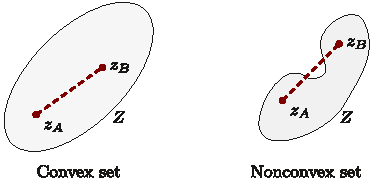
\includegraphics[width=0.4\linewidth]{img/_convex_set.pdf}
        \end{figure}

    \item[Convex function] \marginnote{Convex function}
        Given a convex set $Z \subseteq \mathbb{R}^d$, a function $l: Z \rightarrow \mathbb{R}$ is convex if it holds that:
        \[
            \forall \z_A, \z_B \in Z: \Big( \exists \alpha \in [0, 1]: l(\alpha \z_A + (1-\alpha) \z_B) \leq \alpha l(\z_A) + (1-\alpha) l(\z_B) \Big)
        \]

        \begin{figure}[H]
            \centering
            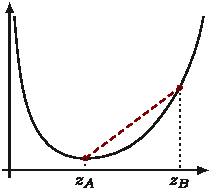
\includegraphics[width=0.25\linewidth]{img/_convex_function.pdf}
        \end{figure}

        \begin{remark}
            Given a differentiable and convex function $l: Z \rightarrow \mathbb{R}$, it holds that any of its points lie above all its tangents:
            \[ \forall \z_A, \z_B \in Z: l(\z_B) \geq l(\z_A) + \nabla l(\z_A)^T (\z_B - \z_A) \]

            \begin{figure}[H]
                \centering
                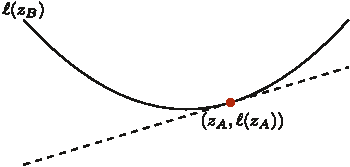
\includegraphics[width=0.3\linewidth]{img/_convex_tangent.pdf}
            \end{figure}
        \end{remark}

    \item[Strongly convex function] \marginnote{Strongly convex function}
        Given a convex set $Z \subseteq \mathbb{R}^d$, a function $l: Z \rightarrow \mathbb{R}$ is strongly convex with parameter $\mu > 0$ if it holds that:
        \[
            \begin{split}
                \forall \z_A, \z_B \in Z, \z_A \neq \z_B: \Big( \exists \alpha \in (0, 1)&: l(\alpha \z_A + (1-\alpha) \z_B) < \\
                &\alpha l(\z_A) + (1-\alpha) l(\z_B) - \frac{1}{2} \mu \alpha (1-\alpha) \Vert \z_A-\z_B \Vert^2 \Big)
            \end{split}
        \]
        Intuitively, it is strictly convex and grows as fast as a quadratic function.

        \begin{remark}
            Given a differentiable and $\mu$-strongly convex function $l: Z \rightarrow \mathbb{R}$, it holds that any of its points lie above all the paraboloids with curvature determined by $\mu$ and tangent to a point of the function:
            \[ \forall \z_A, \z_B \in Z: l(\z_B) \geq l(\z_A) + \nabla l(\z_A)^T (\z_B - \z_A) + \frac{\mu}{2} \Vert \z_B - \z_A \Vert^2 \]

            \begin{figure}[H]
                \centering
                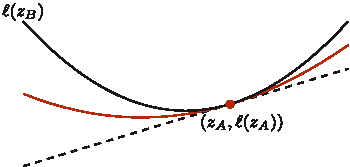
\includegraphics[width=0.35\linewidth]{img/_strongly_convex.pdf}
            \end{figure}

            A geometric interpretation is that strong convexity imposes a quadratic lower-bound to the function.
        \end{remark}
\end{description}

\begin{lemma}[Convexity and gradient monotonicity] \marginnote{Convexity and gradient monotonicity}
    Given a differentiable and convex function $l$, its gradient $\nabla l$ is a monotone operator, which means that it satisfies:
    \[
        \forall \z_A, \z_B: \big( \nabla l(\z_A) - \nabla l(\z_B) \big)^T (\z_A - \z_B) \geq 0
    \]
\end{lemma}

\begin{lemma}[Strict convexity and gradient monotonicity] \marginnote{Strict convexity and gradient monotonicity}
    Given a differentiable and strictly convex function $l$, its gradient $\nabla l$ is a strictly monotone operator, which means that it satisfies:
    \[
        \forall \z_A, \z_B: \big( \nabla l(\z_A) - \nabla l(\z_B) \big)^T (\z_A - \z_B) > 0
    \]
\end{lemma}

\begin{lemma}[Strong convexity and gradient monotonicity] \marginnote{Strong convexity and gradient monotonicity}
    Given a differentiable and $\mu$-strongly convex function $l$, its gradient $\nabla l$ is a strongly monotone operator, which means that it satisfies:
    \[
        \forall \z_A, \z_B: \big( \nabla l(\z_A) - \nabla l(\z_B) \big)^T (\z_A - \z_B) \geq \mu \Vert \z_A - \z_B \Vert^2
    \]
\end{lemma}

\begin{description}
    \item[Lipschitz continuity] \marginnote{Lipschitz continuity}
        Given a function $l$, it is Lipschitz continuous with parameter $L > 0$ if:
        \[
            \forall \z_A, \z_B: \Vert l(\z_A) - l(\z_B) \Vert \leq L \Vert \z_A - \z_B \Vert
        \]

        \begin{remark}
            Given a differentiable function $l$ with $L$-Lipschitz continuous gradient $\nabla l$, it holds that any of its points lie below all the paraboloids with curvature determined by $L$ and tangent to a point of the function:
            \[ \forall \z_A, \z_B \in Z: l(\z_B) \leq l(\z_A) + \nabla l(\z_A)^T (\z_B - \z_A) + \frac{L}{2} \Vert \z_B - \z_A \Vert^2 \]

            \begin{figure}[H]
                \centering
                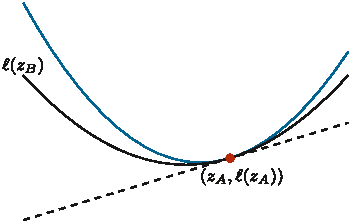
\includegraphics[width=0.35\linewidth]{img/_lipschitz_gradient.pdf}
            \end{figure}

            A geometric interpretation is that Lipschitz continuity of the gradient imposes a quadratic upper-bound to the function.
        \end{remark}
\end{description}

\begin{lemma}[Convexity and Lipschitz continuity of gradient] \marginnote{Convexity and Lipschitz continuity of gradient}
    Given a differentiable convex function $l$ with $L$-Lipschitz continuous gradient $\nabla l$, its gradient is a co-coercive operator, which means that it satisfies:
    \[
        \forall \z_A, \z_B: \Big( \nabla l(\z_A) - \nabla l(\z_B) \Big)^T (\z_A - \z_B) \geq \frac{1}{L} \Vert \nabla l(\z_A) - \nabla l(\z_B) \Vert^2
    \]
\end{lemma}

\begin{lemma}[Strong convexity and Lipschitz continuity of gradient] \marginnote{Strong convexity and Lipschitz continuity of gradient} \phantomsection\label{th:strong_convex_lipschitz_gradient}
    Given a differentiable $\mu$-strongly convex function $l$ with $L$-Lipschitz continuous gradient $\nabla l$, its gradient is a strongly co-coercive operator, which means that it satisfies:
    \[
        \forall \z_A, \z_B: \Big( \nabla l(\z_A) - \nabla l(\z_B) \Big)^T (\z_A - \z_B) \geq \underbrace{\frac{\mu L}{\mu+L}}_{\gamma_1} \Vert \z_A - \z_B \Vert^2 + \underbrace{\frac{1}{\mu+L}}_{\gamma_2} \Vert \nabla l(\z_A) - \nabla l(\z_B) \Vert^2
    \]
\end{lemma}



\section{Iterative descent methods}

\begin{theorem}
    Given a convex function $l$, it holds that a local minimum of $l$ is also global.
    
    Moreover, in the unconstrained optimization case, the first-order necessary condition of optimality is sufficient for a global minimum.
\end{theorem}

\begin{theorem}
    Given a convex function $l$, it holds that $\z^*$ is a global minimum if and only if $\nabla f(\z^*) = 0$.
\end{theorem}


\begin{description}
    \item[Iterative descent] \marginnote{Iterative descent}
        Given a function $l$ and an initial guess $\z^{0}$, an iterative descent algorithm iteratively moves to new points $\z^{k}$ such that:
        \[
            \forall k \in \mathbb{N}: l(\z^{k+1}) < l(\z^{k})
        \]
\end{description}


\subsection{Gradient method}

\begin{description}
    \item[Gradient method] \marginnote{Gradient method}
        Algorithm that given the function $l$ to minimize and the initial guess $\z^0$, computes the update as:
        \[ \z^{k+1} = \z^k - \alpha^k \nabla l(\z^k) \]
        where $\alpha^k > 0$ is the step size and $- \nabla l(\z^k)$ is the step direction.

        \begin{theorem}
            For a sufficiently small $\alpha^k > 0$, the gradient method is an iterative descent algorithm:
            \[ l(\z^{k+1}) < l(\z^{k}) \]

            \begin{proof}
                Consider the first-order Taylor approximation of $l(\z^{k+1})$ about $\z^k$:
                \[
                    \begin{split}
                        l(\z^{k+1}) &= l(\z^k) + \nabla l(\z^k)^T (\z^{k+1} - \z^k) + o(\Vert \z^{k+1} - \z^k \Vert) \\
                        &= l(\z^k) - \alpha^k \Vert \nabla l(\z^k)\Vert^2 + o(\alpha^k)
                    \end{split}
                \]
                Therefore, $l(\z^{k+1}) < l(\z^{k})$ for some $\alpha^k$.
            \end{proof}
        \end{theorem}

        \begin{remark}[Step size choice] \marginnote{Step size choice}
            Possible choices for the step size are:
            \begin{descriptionlist}
                \item[Constant] 
                    $\forall k \in \mathbb{N}: \alpha^k = \alpha > 0$.
                
                \item[Diminishing] 
                    $\alpha^k \overset{k \rightarrow \infty}{\longrightarrow} 0$. To avoid decreasing the step too much, a typical choice is an $\alpha^k$ such that:
                    \[
                        \sum_{k=0}^{\infty} \alpha^k = \infty
                        \qquad
                        \sum_{k=0}^{\infty} (\alpha^k)^2 < \infty
                    \]

                \item[Line search] 
                    Algorithmic methods such as the Armijo rule.
            \end{descriptionlist}
        \end{remark}

    \item[Generalized gradient method] \marginnote{Generalized gradient method}
        Gradient method where the update rule is generalized as:
        \[ \z^{k+1} = \z^k - \alpha^k \matr{D}^k \nabla l(\z^k) \]
        where $\matr{D}^k \in \mathbb{R}^{d \times d}$ is uniformly positive definite (i.e., $\delta_1 \matr{I} \leq \matr{D}^k \leq \delta_2 \matr{I}$ for some $\delta_2 \geq \delta_1 > 0$).

        Possible choices for $\matr{D}^k$ are:
        \begin{itemize}
            \item Steepest descent: $\matr{D}^k = \matr{I}$.
            \item Newton's method: $\matr{D}^k = (\nabla^2 l(\z^k))^{-1}$.
            \item Quasi-Newton method: $\matr{D}^k = (H(\z^k))^{-1}$, where $H(\z^k) \approx \nabla^2 l(\z^k)$.
        \end{itemize}
\end{description}

\begin{description}
    \item[Gradient method as discrete-time integrator with feedback] \marginnote{Gradient method as discrete-time integrator with feedback}
        The gradient method can be interpreted as a discrete-time integrator with a feedback loop. This means that it is composed of:
        \begin{descriptionlist}
            \item[Integrator] A linear system that defines the update: $\z^{k+1} = \z^k - \alpha \vec{u}^k$.
            \item[Plant] A non-linear (bounded) function whose output is re-injected into the integrator. In this case, it is the gradient: $\vec{u}^k = \nabla l(\z^k)$.
        \end{descriptionlist}

        \begin{figure}[H]
            \centering
            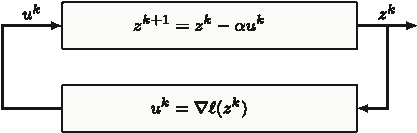
\includegraphics[width=0.55\linewidth]{./img/_gradient_method_integrator.pdf}
        \end{figure}
\end{description} 

\begin{theorem}[Gradient method convergence] \marginnote{Gradient method convergence}
    Consider a function $l$ such that:
    \begin{itemize}
        \item $\nabla l$ is $L$-Lipschitz continuous,
        \item The step size is constant or diminishing. 
    \end{itemize}
    Let $\{ \z^k \}_{k \in \mathbb{N}}$ be the (bounded) sequence generated by the gradient method. It holds that every limit point $\bar{\z}$ of the sequence $\{ \z^k \}_{k \in \mathbb{N}}$ is a stationary point (i.e., $\nabla l(\bar{z}) = 0$).

    In addition, if $l$ is $\mu$-strongly convex and the step size is constant, then the convergence rate of the sequence $\{ \z^k \}_{k \in \mathbb{N}}$ is exponential (also said geometric or linear):
    \[
        \Vert \z^k - \z^* \Vert \leq M \rho^k
    \]
    where $\rho \in (0, 1)$ and $M > 0$ depends on $\mu$, $L$, and $\Vert \z^0 - \z^* \Vert$.

    \begin{proof}
        We need to prove the two parts of the theorem:
        \begin{enumerate}
            \item 
                We want to prove that any limit point of the sequence generated by the gradient method is a stationary point.

                In other words, by considering the gradient method as an integrator with feedback, we want to analyze the equilibrium of the system. Assume that the system converges to some equilibrium $\z_E$. To be an equilibrium, it must be that the feedback loop stopped updating the system (i.e., $\vec{u}^k = 0$ for $k$ after some threshold) so that:
                \[
                    \z_E = \z_E - \alpha \nabla l(\z_E)
                \]
                Therefore, an equilibrium point is necessarily a stationary point of $l$ as it must be that $\nabla l(\z_E) = 0$.
            
            \item 
                We want to prove that if $l$ is $\mu$-strongly convex and the step size is constant, the sequence converges exponentially.

                \begin{remark}
                    As $l$ is convex, its equilibrium is also the global minimum $\z^*$.
                \end{remark}

                Consider the following change in coordinates (i.e., a translation):
                \[ 
                    \begin{gathered}
                        \z^k \mapsto \tilde{\z}^k \\
                        \text{with } \tilde{\z}^k = \z^k - \z_E = \z^k - \z^*
                    \end{gathered}
                \]
                The system in the new coordinates becomes:
                \[
                    \begin{aligned}
                        &\tilde{\z}^{k+1} = \tilde{\z}^k - \alpha \vec{u}^k \\
                        &\begin{aligned}
                            \vec{u}^k &= \nabla l(\z^k) \\
                            &= \nabla l(\tilde{\z}^k + \z^*) \\
                            &= \nabla l(\tilde{\z}^k + \z^*) - \nabla l(\z^*) & & & \text{\small $\nabla l(\z^*)=0$, but useful for \Cref{th:strong_convex_lipschitz_gradient}}
                        \end{aligned}
                    \end{aligned}
                \]

                \begin{figure}[H]
                    \centering
                    \includegraphics[width=0.55\linewidth]{./img/_gradient_method_integrator_new_coords.pdf}
                \end{figure}

                \begin{remark}
                    As $l$ is strongly convex and its gradient Lipschitz continuous, by \Cref{th:strong_convex_lipschitz_gradient} it holds that:
                    \[
                        -(\vec{u}^k)^T \tilde{\z}^k \leq - \gamma_1 \Vert \tilde{\z}^k \Vert^2 - \gamma_2 \Vert \tilde{\vec{u}}^k \Vert^2
                    \]
                \end{remark}

                Consider a Lyapunov function $V: \mathbb{R}^d \rightarrow \mathbb{R}_{\geq 0}$ defined as:
                \[
                    V(\tilde{\z}) = \Vert \tilde{\z} \Vert^2
                \]
                It holds that:
                \[
                    \begin{aligned}
                        V(\tilde{\z}^{k+1}) - V(\tilde{\z}^k) &= \Vert \tilde{\z}^{k+1} \Vert^2 - \Vert \tilde{\z}^k \Vert^2 \\
                        &= \cancel{\Vert \tilde{\z}^k \Vert^2} - 2\alpha(\vec{u}^k)^T\tilde{\z}^k + \alpha^2 \Vert \vec{u}^k \Vert^2 - \cancel{\Vert \tilde{\z}^k \Vert^2} &&& \text{\Cref{th:strong_convex_lipschitz_gradient}} \\
                        &\leq -2\alpha\gamma_1 \Vert\tilde{\z}^k\Vert^2 + \alpha(\alpha-2\gamma_2) \Vert\vec{u}^k\Vert^2
                    \end{aligned}
                \]

                By choosing $\alpha \leq 2\gamma_2$, we have that:
                \[
                    \begin{split}
                        V(\tilde{\z}^{k+1}) - V(\tilde{\z}^k) &\leq -2\alpha\gamma_1 \Vert \tilde{\z}^k \Vert^2 \\
                        \iff \Vert \tilde{\z}^{k+1} \Vert^2 - \Vert \tilde{\z}^k \Vert^2 &\leq -2\alpha\gamma_1 \Vert \tilde{\z}^k \Vert^2 \\
                        \iff \Vert \tilde{\z}^{k+1} \Vert^2 &\leq (1-2\alpha\gamma_1) \Vert \tilde{\z}^k \Vert^2 \\
                    \end{split}
                \]
                Finally, as the gradient method is an iterative descent algorithm, it holds that:
                \[
                    \begin{split}
                        \Vert \tilde{\z}^{k+1} \Vert^2 &\leq (1-2\alpha\gamma_1) \Vert \tilde{\z}^k \Vert^2 \\
                        &\leq \dots \\
                        &\leq (1-2\alpha\gamma_1)^k \Vert \tilde{\z}^0 \Vert^2 \\
                    \end{split}
                \]
                Therefore, the sequence $\{ \tilde{\z}^k \}_{k \in \mathbb{R}}$ goes exponentially fast to zero and we have shown that:
                \[
                    \begin{split}
                        \Vert \z^{k+1} - \z^* \Vert^2 &\leq (1-2\alpha\gamma_1)^k \Vert \z^0 - \z^* \Vert^2 \\
                        &= \rho^k M
                    \end{split}
                \]
        \end{enumerate}
    \end{proof}
\end{theorem}

\begin{remark}[Gradient method for a quadratic function] \marginnote{Gradient method for a quadratic function}
    Given the problem of minimizing a quadratic function:
    \[
        \min_{\z} \frac{1}{2}\z^T \matr{Q} \z + \vec{r}^T \z
        \qquad
        \nabla l = \matr{Q} \z^k + \vec{r}
    \]
    The gradient method can be reduced to an affine linear system:
    \[
        \begin{split}
            \z^{k+1} &= \z^k - \alpha (\matr{Q} \z^k + \vec{r}) \\
            &= (\matr{I} - \alpha \matr{Q}) \z^k - \alpha \vec{r}
        \end{split}
    \]
    For a sufficiently small $\alpha$, the matrix $(\matr{I} - \alpha \matr{Q})$ is Schur (i.e., $\forall \matr{\rho}, |\matr{\rho}| < 1: \sum_{i=0}^{\infty} \matr{\rho}^i = (1-\matr{\rho})^{-1}$). Therefore, the solution can be computed in closed form as:
    \[
        \begin{split}
            \z^k &= (\matr{I} - \alpha \matr{Q})^k \z^0 - \alpha \sum_{\tau=0}^{k-1} (\matr{I} - \alpha \matr{Q})^\tau \vec{r} \\
            &\overset{k \rightarrow \infty}{\longrightarrow} - \alpha \left( \sum_{\tau=0}^{\infty} (\matr{I} - \alpha \matr{Q})^\tau \right) \vec{r} = -\matr{Q}^{-1} \vec{r}
        \end{split}
    \]
\end{remark}

\begin{remark}[Gradient flow] \marginnote{Gradient flow}
    By inverting the integrator and plant of the discrete-time integrator of the gradient method, and considering the continuous-time case, the result is the gradient flow:
    \[
        \dot{\z}(t) = -\nabla l(\z(t))
    \]
    which has a solution if the vector field is Lipschitz continuous.

    \begin{figure}[H]
        \centering
        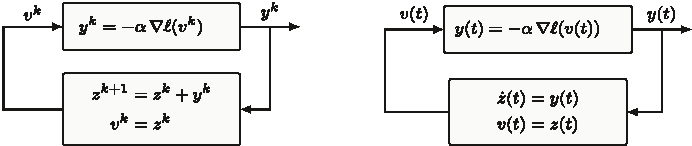
\includegraphics[width=0.8\linewidth]{./img/_gradient_flow.pdf}
    \end{figure}
\end{remark}


\subsection{Accelerated gradient methods}

\begin{description}
    \item[Heavy-ball method] \marginnote{Heavy-ball method}
        Given $\eta^0$ and $\eta^{-1}$, the algorithm is defined as:
        \[
            \eta^{k+1} = \eta^k + \alpha_1 (\eta^k - \eta^{k-1}) - \alpha_2 \nabla l(\eta^k)
        \]
        with $\alpha_1, \alpha_2 > 0$.

        \begin{remark}
            With $\alpha_1 = 0$, the algorithm is reduced to the gradient method with step size $\alpha_2$.
        \end{remark}

        \begin{remark}
            The algorithm admits a state-space representation as a discrete-time integrator with a feedback loop:
            \begin{figure}[H]
                \centering
                \includegraphics[width=0.55\linewidth]{./img/_heavy_ball.pdf}
            \end{figure}

            Note that the matrix $\begin{bmatrix} 1+\alpha_1 & -\alpha_1 \\ 1 & 0 \end{bmatrix}$ is row stochastic.
        \end{remark}

    \item[Generalized heavy-ball method] \marginnote{Generalized heavy-ball method}
        Given $\zeta^0$ and $\zeta^{-1}$, the algorithm is defined as:
        \[
            \zeta^{k+1} = \zeta^k + \alpha_1 (\zeta^k - \zeta^{k-1}) - \alpha_2 \nabla l(\zeta^k + \alpha_3(\zeta^k - \zeta^{k-1}))
        \]
        with $\alpha_1, \alpha_2, \alpha_3 > 0$.

        \begin{remark}
            The algorithm admits a state-space representation as a discrete-time integrator with a feedback loop:
            \begin{figure}[H]
                \centering
                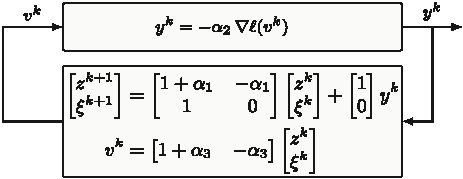
\includegraphics[width=0.55\linewidth]{./img/_generalized_heavy_ball.pdf}
            \end{figure}
        \end{remark}
\end{description}



\section{Parallel optimization}


\begin{description}
    \item[Cost-coupled optimization] \marginnote{Cost-coupled optimization}
        Problem of minimizing $N$ cost functions $l_i: \mathbb{R}^d \rightarrow \mathbb{R}$, each local and private to an agent:
        \[
            \min_{\z \in \mathbb{R}^{d}} \sum_{i=1}^{N} l_i(\z)
        \]
    
    \item[Batch gradient method] \marginnote{Batch gradient method}
        Compute the gradient method direction by considering all the losses:
        \[
            \z^{k+1} = \z^k - \alpha \sum_{i=1}^{N} \nabla l_i(\z^k)
        \]

        \begin{remark}
            Computation in this way can be expensive.
        \end{remark}

    \item[Incremental gradient method] \marginnote{Incremental gradient method}
        At each iteration $k$, compute the direction by considering the loss of a single agent $i^k$:
        \[
            \z^{k+1} = \z^k - \alpha \nabla l_{i^k}(\z^k)
        \]

        \begin{remark}
            Two possible rules to select the agent at each iteration are:
            \begin{descriptionlist}
                \item[Cyclic] 
                    $i^k = 1, 2, \dots, N, 1, 2, \dots, N, \dots$
                \item[Randomized] 
                    Draw $i^k$ from a uniform distribution.
            \end{descriptionlist}
        \end{remark}
        % \begin{remark}
        %     The step size should decrease to reach convergence.
        % \end{remark}
\end{description}
    \chapter{Formation control}


\section{Intuition with mass-spring systems}

\begin{description}
    \item[Mass-spring system] \marginnote{Mass-spring system}
        System of $N$ masses where each mass $i$ has a position $x_i \in \mathbb{R}$ and is connected through a sprint to mass $i-1$ and $i+1$. Each spring has an elastic constant $a_{j, i} = a_{i, j} > 0$.

        \begin{figure}[H]
            \centering
            \includegraphics[width=0.5\linewidth]{./img/mass_spring_system.png}
        \end{figure}

        The elastic force $F_{e,i}(x)$ at mass $i$ is given by:
        \[
            F_{e,i}(x) = -a_{i,i-1}(x_i-x_{i-1}) - a_{i,i+1}(x_i - x_{i+1})
        \]
        Equivalently, it is possible to express the elastic force as the negative gradient of the elastic potential energy:
        \[
            F_{e,i}(x) = -\frac{\partial}{\partial x_i}\left( \frac{1}{2} a_{i,i-1} \Vert x_i - x_{i-1} \Vert^2 + \frac{1}{2} a_{i,i+1} \Vert x_i - x_{i+1} \Vert^2 \right)
        \]

    \item[Mass-spring system with two springs] \marginnote{Mass-spring system with two springs}
        Assume that the springs of a mass-spring system can be split with halved elastic constants.
        \begin{figure}[H]
            \centering
            \includegraphics[width=0.5\linewidth]{./img/mass_spring_system2.png}
        \end{figure}

        Accordingly, the elastic force can be defined as:
        \[
            \small
            \begin{split}
                F_{e,i}(x) 
                &= 
                    - \frac{1}{2} a_{i,i-1}(x_i - x_{i-1}) 
                    - \frac{1}{2} a_{i-1,i}(x_i - x_{i-1}) 
                    - \frac{1}{2} a_{i,i+1}(x_i - x_{i+1}) 
                    - \frac{1}{2} a_{i+1,i}(x_i - x_{i+1}) \\
                &= 
                    - \frac{1}{2} a_{i,i-1}(x_i - x_{i-1}) 
                    + \frac{1}{2} a_{i-1,i}(x_{i-1} - x_i) 
                    - \frac{1}{2} a_{i,i+1}(x_i - x_{i+1}) 
                    + \frac{1}{2} a_{i+1,i}(x_{i+1} - x_i) \\
                &= -\frac{\partial}{\partial x_i} \left( 
                    \frac{1}{2} \frac{a_{i,i-1}}{2} \Vert x_i - x_{i-1} \Vert^2 + 
                    \frac{1}{2} \frac{a_{i-1,i}}{2} \Vert x_{i-1} - x_{i} \Vert^2 + 
                    \frac{1}{2} \frac{a_{i,i+1}}{2} \Vert x_i - x_{i+1} \Vert^2 + 
                    \frac{1}{2} \frac{a_{i+1,i}}{2} \Vert x_{i+1} - x_{i} \Vert^2 \right)
            \end{split}
        \]
        The total potential energy (i.e., sum of the function in the derivative over all masses) can be compactly defined as:
        \[
            \begin{split}
                V(x) &= \sum_{i=1}^{N} \sum_{j \in \mathcal{N}_i} \frac{1}{2} \frac{a_{i,j}}{2} \Vert x_i - x_j \Vert^2 \\
                &= \sum_{i=1}^{N} \sum_{j \in \mathcal{N}_i} V_{ij}(x_i, x_j)
            \end{split}
            \quad
            V_{i,j}(x_i, x_j) = \frac{1}{2} \frac{a_{i,j}}{2} \Vert x_i - x_j \Vert^2
        \]
        where $\mathcal{N}_i = \{ i-1, i+1 \}$.

        Then, the potential energy at mass $i$ can be written as:
        \[
            V_i(x) = \sum_{j \in \mathcal{N}_i} ( V_{i,j}(x_i, x_j) + V_{j,i}(x_j, x_i) )
        \]
            
        Finally, the elastic force at mass $i$ can be reformulated as:
        \[
            \begin{split}
                F_{e,i}(x) 
                &= - \frac{\partial}{\partial x_i} \Big( V_{i,i-1}(x_i, x_{i-1}) + V_{i-1,i}(x_{i-1}, x_i) + V_{i,i+1}(x_i, x_{i+1}) + V_{i+1,i}(x_{i+1}, x_i) \Big) \\
                &= - \frac{\partial}{\partial x_i} \left( \sum_{j \in \mathcal{N}_i} ( V_{i,j}(x_i, x_j) + V_{j,i}(x_j, x_i) ) \right) \\
                &= - \frac{\partial}{\partial x_i} V_i(x) \\
                &= - \frac{\partial}{\partial x_i} V(x)
            \end{split}
        \]

        \begin{remark}
            The system can be generalized to a graph of interconnected masses.

            \begin{figure}[H]
                \centering
                \includegraphics[width=0.3\linewidth]{./img/mass_spring_system3.png}
            \end{figure}
        \end{remark}
        
        By adding a constant damping coefficient (i.e., dispersion of velocity) $c=1$, the overall system dynamics can be defined as:
        \[
            \begin{split}
                \dot{x}_i &= v_i \\
                m_i \dot{v}_i &= - v_i - c\frac{\partial}{\partial x_i} V(x) = - v_i - \frac{\partial}{\partial x_i} V(x)
            \end{split}
        \]
        where $m_i$ is the mass of the $i$-th mass.

        By assuming small masses $m_i$, the following approximation can be made:
        \[
            \begin{gathered}
                \cancel{m_i \dot{v}_i} = - v_i - \frac{\partial}{\partial x_i} V(x) \Rightarrow v_i \approx -\frac{\partial}{\partial x_i} V(x) \\
                \dot{x_i} = -\frac{\partial}{\partial x_i} V(x) = F_{e,i}(x)
            \end{gathered}
        \]

        By more explicitly expanding the dynamics of the $i$-th mass, we have that:
        \[
            \begin{aligned}
                \dot{x}_i
                &= - \sum_{j \in \mathcal{N}_i} \frac{\partial}{\partial x_i} \Big( V_{i,j}(x_i, x_j) + V_{j,i}(x_j, x_i) \Big) \\
                &= - \sum_{j \in \mathcal{N}_i} \frac{\partial}{\partial x_i} \left( \frac{1}{2} \frac{a_{i,j}}{2} \Vert x_i - x_j \Vert^2 + \frac{1}{2} \frac{a_{j,i}}{2} \Vert x_j - x_i \Vert^2 \right) \\
                &= - \sum_{j \in \mathcal{N}_i} \left( \frac{1}{2} a_{i,j} (x_i - x_j) - \frac{1}{2} a_{j,i} (x_j - x_i) \right) &&& \text{\footnotesize $a_{i,j}=a_{j,i}$ ($G$ undirected)} \\
                &= - \sum_{j \in \mathcal{N}_i} a_{i,j} (x_i - x_j) &&& \text{\footnotesize i.e., Laplacian dynamics}
            \end{aligned}
        \]
        
        Therefore, the overall system follows a Laplacian dynamics and can be equivalently formulated as the gradient flow of $V$:
        \[
            \begin{split}
                \dot{\x} &= -\matr{L}\x = - \nabla V(x) \\
                \begin{bmatrix}
                    \dot{x}_1 \\ \vdots \\ \dot{x}_N
                \end{bmatrix}
                &=
                - \begin{bmatrix}
                    \frac{\partial}{\partial x_1} V(x) \\
                    \vdots
                    \\
                    \frac{\partial}{\partial x_N} V(x)
                \end{bmatrix}
            \end{split}
        \]
        And consensus is reached at a stationary point of $V(x)$.
\end{description}



\section{Formation control based on potential functions}


\begin{remark}
    The gradient flow based on the global potential function/energy can be computed in a distributed way (i.e., it depends only on neighboring states):
    \[
        \dot{x}_i(t) = - \sum_{j \in \mathcal{N}_i} \frac{\partial}{\partial x_i} \Big( V_{i,j}(x_i, x_j) + V_{j,i}(x_j, x_i) \Big)
    \]
\end{remark}


\begin{description}
    \item[Formation control] \marginnote{Formation control}
        Consider $N$ agents with states $\x_i(t) \in \mathbb{R}^d$ and communicating according to a fixed undirected graph $G$. The goal is to position each agent respecting the desired distances $d_{ij} = d_{ji}$ between them:
        \[
            \forall (i,j) \in E: \Vert \x_i^\text{form} - \x_j^\text{form} \Vert = d_{ij}
        \]

        To solve the problem, the potential function can be defined as:
        \[
            \begin{gathered}
                V^\text{form}(\x) = \sum_{i=1}^{N} \sum_{j \in \mathcal{N}_i} V_{ij}^\text{form}(\x_i, \x_j) \\
                V_{ij}^\text{form}(\x_i, \x_j) = \frac{1}{8} \left( \Vert \x_i - \x_j \Vert^2 - d_{ij}^2 \right)^2
            \end{gathered}
        \]
        where $\frac{1}{8}$ is used to cancel out the fraction when deriving.

        The gradient flow dynamics is then:
        \[
            \begin{split}
                \dot{\x}_i &= - \sum_{j \in \mathcal{N}_i} \frac{\partial}{\partial \x_i} \left( V_{ij}^\text{form}(\x_i, \x_j) + V_{ji}^\text{form}(\x_j, \x_i) \right) \\
                &= - \sum_{j \in \mathcal{N}_i} \left( \Vert \x_i - \x_j \Vert^2 - d_{ij}^2 \right)(\x_i - \x_j)
            \end{split}
        \]

        \begin{remark}
            Apart from the desired formation, another equilibrium of this dynamics is $x_1 = x_2 = \dots = x_N$ (i.e., a collision).
        \end{remark}

    \item[Collision avoidance potential function/Barrier function] \marginnote{Collision avoidance potential function/Barrier function}
        Function $V_{ij}^\text{ca}(\x_i, \x_j)$ such that:
        \[
            \lim_{\Vert \x_i - \x_j \Vert \rightarrow 0} V_{ij}^\text{ca}(\x_i, \x_j) = +\infty
        \]

        \begin{remark}
            A possible barrier function is:
            \[
                V_{ij}^\text{ca}(\x_i, \x_j) = - \log( \Vert \x_i - \x_j \Vert^2 - d^2 )
            \]
            where $d$ is the safety distance.
        \end{remark}

    \item[Formation control with obstacle avoidance] \marginnote{Formation control with obstacle avoidance}
        Formation control where agents avoid collisions and obstacles. The dynamics is:
        \[
            \dot{\x}_i = - \frac{\partial}{\partial \x_i} \Big( V^\text{form}(\x) + V^\text{ca}(\x) + V^\text{obs}(\x) \Big)
        \]
        where:
        \begin{itemize}
            \item $V^\text{ca}(\x) = \sum_{i=1}^N \sum_{j \in \mathcal{N}_i} V_{ij}^\text{ca}(\x_i, \x_j)$ and $V_{ij}^\text{ca}(\x_i, \x_j)$ is the barrier function to avoid collisions between agents.
            \item $V^\text{obs}(\x) = \sum_{i=1}^N V_{i}^\text{obs}(\x_i)$ and $V_{i}^\text{obs}(\x_i)$ is the barrier function to avoid collisions between an agent and an obstacle.
        \end{itemize}
\end{description}



    \chapter{Cooperative robotics}


\begin{description}
    \item[Cooperative robotics] \marginnote{Cooperative robotics}
        Problem where $N$ agents want to optimize their positions $\z_i \in \mathbb{R}^2$ to perform multi-robot surveillance in an environment with:
        \begin{itemize}
            \item A static target to protect $\r_0 \in \mathbb{R}^2$.
            \item Static intruders/opponents $\r_i \in \mathbb{R}^2$, each assigned to an agent $i$.
        \end{itemize}

        The average position of the agents define the barycenter:
        \[ \sigma(\z) = \frac{1}{N} \sum_{i=1}^N \z_i \]

        The local cost function of agent $i$ is:
        \[
            l_i(\z_i, \sigma(\z)) = 
            \gamma_i \underbrace{\Vert \z_i - \r_i \Vert^2}_{\text{close to opponent}} + 
            \underbrace{\Vert \sigma(\z) - \r_0 \Vert^2}_{\text{barycenter close to protectee}}
        \]
        Note that the opponent component only depends on local variables while the target component needs global information.

        \begin{remark}
            The barycenter $\sigma(\z): \mathbb{R}^{2N} \rightarrow \mathbb{R}^{2}$ can be seen as an aggregation function.
        \end{remark}

        \begin{remark}
            A scenario that this formulation fails to handle is when the agents are placed symmetrically and moves symmetrically as the barycenter remains the same even if the agents move farther away.
        \end{remark}
\end{description}



\section{Aggregative optimization}

\begin{description}
    \item[Aggregative optimization] \marginnote{Aggregative optimization}
        Problem defined as:
        \[
            \min_{\z_1, \dots, \z_N} \sum_{i=1}^{N} l_i(\z_i, \sigma(\z))
        \]
        where:
        \begin{itemize}
            \item $\z = (\z_1, \dots, \z_N)$ with $\z_i \in \mathbb{R}^{n_i}$,
            \item $l_i: \mathbb{R}^{n_i} \rightarrow \mathbb{R}^d$ is the loss function of the agent $i$,
            \item $\sigma(\z)$ is an aggregation function generically defined as $\sigma(\z) = \frac{1}{N} \sum_{i=1}^{N} \phi_i(\z_i)$, for some $\phi_i: \mathbb{R}^{n_i} \rightarrow \mathbb{R}^d$
        \end{itemize}

    \item[Distributed aggregative optimization] \marginnote{Distributed aggregative optimization}
        Distributed case of aggregative optimization where each agent has only access to the loss $l_i$, the operator of the aggregation function $\phi_i$, and the position $\z_i$ of itself and its neighbors.
\end{description}

\begin{remark}
    The goal of the task is not to reach consensus among agents.
\end{remark}


\subsection{Centralized gradient method}

\begin{description}
    \item[Centralized gradient method (scalar)] \marginnote{Centralized gradient method (scalar)}
        Consider $N$ agents with $z_i \in \mathbb{R}$ and $\sigma: \mathbb{R}^N \rightarrow \mathbb{R}$. The update step, assuming global access to the parameters, can be performed as:
        \[
            z_i^{k+1} = z_i^k - \alpha \frac{\partial}{\partial z_i} \left.\left( \sum_{j=1}^{N} l_j(z_j, \sigma(z_1, \dots, z_N)) \right) \right|_{z_j=z_j^k}
        \]
        By expanding the derivative, we have that:
        \[
            \begin{split}
                &\frac{\partial}{\partial z_i} \left.\left( \sum_{j=1}^{N} l_j(z_j, \sigma(z_1, \dots, z_N)) \right) \right|_{z_j=z_j^k} \\
                &= 
                    \left.\frac{\partial}{\partial z_i} l_i(z_i, \sigma) \right|_{\substack{z_i = z_i^k,\\\sigma = \sigma(\z^k)}} + 
                    \left.\left(\sum_{j=1}^{N} \frac{\partial}{\partial \sigma} l_j(z_j, \sigma) \right)\right|_{\substack{z_j = z_j^k,\\\sigma = \sigma(\z^k)}} \cdot
                    \left.\frac{\partial}{\partial z_i} \sigma(z_1, \dots, z_N)\right|_{\substack{z_j=z_j^k}}
            \end{split}
        \]

    \item[Centralized gradient method (vector)] \marginnote{Centralized gradient method (vector)}
        Generalized to the vector case, the update step becomes:
        \[
            \z_i^{k+1} = \z_i^k - \alpha \left[ \nabla \left.\left( \sum_{j=1}^{N} l_j(\z_j, \sigma(\z_1, \dots, \z_N)) \right) \right|_{\z_j=\z_j^k} \right]_{(i)}
        \]
        And the gradient can be expanded as:
        \[
            \begin{split}
                &\left[ \nabla \left.\left( \sum_{j=1}^{N} l_j(\z_j, \sigma(\z_1, \dots, \z_N)) \right) \right|_{\z_j=\z_j^k} \right]_{(i)} \\
                &= 
                    \left.\nabla_{[\z_i]} l_i(\z_i, \sigma)\right|_{\substack{\z_i=\z_i^k,\\\sigma=\sigma(\z^k)}} +
                    \left.\sum_{j=1}^{N} \nabla_{[\sigma]} l_j(\z_j, \sigma)\right|_{\substack{\z_j=\z_j^k\\\sigma=\sigma(\z^k)}} \cdot
                    \left.\frac{1}{N}\nabla \phi_i(\z_i)\right|_{\z_i=\z_i^k} 
            \end{split}
        \]
        where $\nabla_{[\z_i]} l_i(\z_i, \sigma)$ is the gradient w.r.t. the first argument and $\nabla_{[\sigma]} l_i(\z_i, \sigma)$ is w.r.t. the second one.
\end{description}


\subsection{Aggregative tracking distributed optimization algorithm}

\begin{description}
    \item[Aggregative tracking distributed optimization algorithm] \marginnote{Aggregative tracking distributed optimization algorithm}
    Algorithm where each agent $i$ has:
    \begin{itemize}
        \item An estimate $\z_i^k$ of its optimal position $\z_i^*$,
        \item An estimate $\s_i^k$ of the aggregation function $\sigma(\z^k) = \frac{1}{N} \sum_{j=1}^{N} \phi_j(\z_j^k)$,
        \item An estimate $\v_i^k$ of the gradient with respect to the second argument of the loss $\sum_{j=1}^{N} \nabla_{[\sigma(\z^k)]} l_j(\z_j^k, \sigma(\z^k))$.
    \end{itemize}

    The step is based on the centralized gradient method using the local estimates:
    \[
        \begin{aligned}
            \z_i^{k+1} &= \z_i^k - \alpha \left( \nabla_{[\z_i]} l_i(\z_i^k, \s_i^k) + \v_i^k \nabla \phi_i(\z_i^k) \right) && \z_i^0 \in \mathbb{R}^{n_i} \\
            \s_i^{k+1} &= \sum_{j \in \mathcal{N}_i} a_{ij} \s_j^k + \left( \phi_i(\z_i^{k+1}) - \phi_i(\z_i^k) \right) && \s_i^0 = \phi_i(\z_i^0) \\
            \v_i^{k+1} &= \sum_{j \in \mathcal{N}_i} a_{ij} \v_j^k + \left( \nabla_{[\s_i^{k+1}]} l_i(\z_i^{k+1}, \s_i^{k+1}) - \nabla_{[\s_i^k]} l_i(\z_i^k, \s_i^k) \right) && \v_i^0 = \nabla_{[\s_i^0]} l_i(\z_i^0, \s_i^0) \\
        \end{aligned}
    \]
    where the estimates $\s_i^k$ and $\v_i^k$ are obtained through dynamic average consensus (\Cref{sec:gradient_tracking_algorithm}).

    \begin{remark}
        $\v_i^k$ is a double approximation as it uses $\s_i^{k+1}$ and $\s_i^k$ instead of the real $\sigma$.
    \end{remark}

    \begin{theorem}[Aggregative tracking distributed optimization algorithm convergence]
        If:
        \begin{itemize}
            \item The communication digraph $G$ is strongly connected and aperiodic, and $\matr{A}$ is doubly stochastic,
            \item $\sum_{i=1}^{N} l_i(\cdot, \sigma(\cdot))$ strongly convex with $\phi_i(\cdot)$ differentiable and Lipschitz continuous.
            \item $\nabla_{[\z]} l_i(\cdot, \cdot)$, $\nabla_{[\sigma]} l_i(\cdot, \cdot)$, and $\nabla \phi_i(\cdot) \nabla_{[\sigma]} l_i(\cdot, \cdot)$ are Lipschitz continuous.
        \end{itemize}
        Then, there exists an $\alpha^*$ such that, for any step size $\alpha \in (0, \alpha^*)$, the sequences of local estimates $\{ \z_i^k, \dots, \z_N^k \}_{k \in \mathbb{N}}$ generated using the aggregative tracking distributed optimization algorithm converge to the optimal solution at a linear rate:
        \[
            \lim_{k \rightarrow \infty} \Vert \z_i^k - \z_i^* \Vert = 0
        \]
    \end{theorem}

    % \begin{remark}
    %     LTI:
    %     \[
    %         \begin{aligned}
    %             \z_i^{k+1} = \z_i^k - \alpha() \\
    %             \begin{aligned}
    %                 s_i^{k+1} &= \sum_{j=1}^{N} a_i s_j^k + ... \\
    %                 v_i^{k+1} &=
    %             \end{aligned}
    %         \end{aligned}
    %     \]  

    %     Upper part is a ``slow'' system

    %     Lower part is a ``fast'' system
    % \end{remark}
\end{description}


\subsection{Online aggregative optimization}

\begin{description}
    \item[Online aggregative optimization] \marginnote{Online aggregative optimization}
        Time-varying case of aggregative optimization where intruders also move. The problem can be defined as:
        \[
            \min_{\z=(\z_1, \dots, \z_N)} \sum_{i=1}^{N} l_i^k(\z_i, \sigma^k(\z)) \quad\text{subject to $\z_i \in Z_i^k$}
        \]
        where $Z_i^k$ is a closed convex set.

        \begin{remark}
            As intruders are dynamic, the optimum of each agent $\z_i^{k,*}$ changes over time.
        \end{remark}

    \item[Projected aggregative tracking] \marginnote{Projected aggregative tracking}
        Algorithm for online aggregative optimization defined as:
        \[
            \begin{aligned}
                \tilde{\z}_i^k &= P_{Z_i^k} \left[ \z_i^k - \alpha \big( \nabla_{[\z_i^k]} l_i^k(\z_i^k, \s_i^k) + \v_i^k \nabla\phi_i^k(\z_i^k) \big) \right] \\
                \z_i^{k+1} &= \z_i^k + \delta(\tilde{\z}_i^k - \z_i^k) && \z_i^0 \in \mathbb{R}^{n_i} \\
                \s_i^{k+1} &= \sum_{j \in \mathcal{N}_i} a_{ij} \s_j^k + \left( \phi^{k+1}_i(\z_i^{k+1}) - \phi^{k}_i(\z_i^k) \right) && \s_i^0 = \phi_i(\z_i^0) \\
                \v_i^{k+1} &= \sum_{j \in \mathcal{N}_i} a_{ij} \v_j^k + \left( \nabla_{[\s_i^{k+1}]} l_i^{k+1}(\z_i^{k+1}, \s_i^{k+1}) - \nabla_{[\s_i^k]} l_i^k(\z_i^k, \s_i^k) \right) && \v_i^0 = \nabla_{[\s_i^0]} l_i(\z_i^0, \s_i^0) \\
            \end{aligned}
        \]
        where $P_{Z_i^k}$ is the Euclidean projection and $\delta \in (0, 1)$ is a hyperparameter.
\end{description}
    \chapter{Multi-robot safety controllers}


\begin{description}
    \item[Control-affine non-linear dynamical system] \marginnote{Control-affine non-linear dynamical system}
        System whose dynamics follows:
        \[
            \dot{\x}(t) = f(\x(t)) + g(\x(t)) \u(t) \quad \x(0) = \x_0
        \]
        with $\x(t) \in \mathbb{R}^n$, $\u(t) \in U \subseteq \mathbb{R}^m$, $f(\x(t)) \in \mathbb{R}^n$, and $g(\x(t)) \in \mathbb{R}^{n \times m}$.

        $f(\x(t))$ can be seen as the drift of the system and $\u(t)$ a coefficient that controls how much $g(\x(t))$ is injected into $f(\x(t))$.

        The overall system can be interpreted as composed of:
        \begin{itemize}
            \item A high-level controller that produces the direction $\u^\text{ref}(\x)$ towards the target position.
            \item A safety layer that modifies $\u^\text{ref}(\x)$ into $\u(t) = \kappa(\x)$ to account for obstacles.
        \end{itemize}

    \item[Safety control] \marginnote{Safety control}
        Given a (sufficiently regular) function $V^s: X \subseteq \mathbb{R}^n \rightarrow \mathbb{R}$, it is possible to define a safe state set as:
        \[
            X^s = \{ \x \in X \subseteq \mathbb{R}^n \mid V^s(\x) \geq 0 \}
        \]

        The goal is to design a feedback control law $\kappa^s: X \rightarrow \mathbb{R}^m$ for a control-affine non-linear dynamical system such that the set $X^s$ is forward invariant (i.e., any trajectory starting in $X^s$ remains in $X^s$).

        \begin{figure}[H]
            \centering
            \includegraphics[width=0.25\linewidth]{./img/safety_control.png}
        \end{figure}

        \begin{remark}
            The time derivative of $V^s(\x(t))$ along the system trajectories is given by:
            \[
                \begin{split}
                    \frac{d}{dt} V^s(\x(t)) 
                    &= \nabla V^s(\x(t))^T \frac{d}{dt} \x(t) \\
                    &= \nabla V^s(\x(t))^T \Big( f(\x(t)) + g(\x(t)) \u(t) \Big) \\
                    &= \nabla V^s(\x(t))^T f(\x(t)) + \sum_{h=1}^{m} \Big( \nabla V^s(\x(t))^T g_h(\x(t)) \u_h(t) \Big)\\
                    &= L_f V^s(\x(t)) + L_g V^s(\x(t)) \u(t) \\
                \end{split}
            \]
            where $L_h V^s(\x(t)) = \nabla V^s(\x(t))^T h(\x(t))$ is the lie derivative.
        \end{remark}

    \item[Control barrier function (CBF)] \marginnote{Control barrier function (CBF)}
        A function $V^s$ is a control barrier function if there exists a continuous strictly increasing function $\gamma: \mathbb{R} \rightarrow \mathbb{R}$ with $\gamma(0) = 0$ such that the following inequality (control barrier certificate) holds:
        \[
            \sup_{\u \in U} \{ L_fV^s(\x) + L_gV^s(\x)\u + \gamma(V^s(\x)) \} \geq 0 \quad \forall \x \in X
        \]
        $\gamma$ can be interpreted as a degree of movement freedom since, as long as it holds that $V^s(\x(t)) > 0$, it is allowed that $\frac{d}{dt} V^s(\x(t)) < 0$ (i.e., the agent can move closer to the border between safe and unsafe region).

        \begin{remark}
            In principle, the negative part of $\gamma$ is not necessary (the agent should start in a safe area). However, as it is strictly increasing, it allows to move out the unsafe region if the agent ever ends up there.
        \end{remark}

        \begin{example}
            A simple choice for $\gamma$ is a linear function $\gamma(r) = \gamma r$ with $\gamma > 0$.
        \end{example}

    \item[Set of admissible safe controllers] \marginnote{Set of admissible safe controllers}
        The set of inputs that satisfy the control barrier certificate for a given state $\x$ is:
        \[
            U^s(\x) = \{ \u \in U \mid L_f V^s(\x) + L_g V^s(\x) \u + \gamma(V^s(\x)) \geq 0 \}
        \]
\end{description}


\section{Safety filter via control barrier certificate}

\begin{description}
    \item[Safety filter via control barrier certificate] \marginnote{Safety filter via control barrier certificate}
        Given a possibly unsafe reference input (from the high-level controller) $\u^\text{ref}(\x) \in \mathbb{R}^m$, the safety controller (i.e., rectifying controller) based on the control barrier certificate is designed to be minimally invasive (i.e., alter the reference as little as possible). 
        
        The policy $\u = \kappa^s(\x)$ can be defined as:
        \[
            \begin{gathered}
                \kappa^s(\x) = \arg\min_{\u \in U} \Vert \u - \u^\text{ref}(\x) \Vert^2 \\
                \text{subject to } -L_fV^s(\x) - L_gV^s(\x)\u - \gamma(V^s(\x)) \leq 0
            \end{gathered}
        \]

        \begin{remark}
            In the general case, this problem should be solved at each $t \geq 0$.
        \end{remark}


    \item[Single integrator model] \marginnote{Single integrator model}
        Control-affine non-linear dynamical system where $f(\x(t)) = 0$ and $g(\x(t)) = \matr{I}$. The dynamics is:
        \[
            \begin{split}
                \dot{\x} 
                &= 0 + \matr{I}\u \\ 
                &= \u
            \end{split}
        \]
        with $\x \in \mathbb{R}^d$ and $\u \in \mathbb{R}^d$.

        \begin{remark}
            In the case of single integrators, we have that:
           \begin{itemize}
            \item $L_f V^s(\x) = \nabla V^s(\x)^T 0 = 0$,
            \item $L_g V^s(\x) = \nabla V^s(\x)^T \matr{I} = \nabla V^s(\x)^T$.
           \end{itemize}
           Therefore:
           \[
                \begin{split}
                    \frac{d}{dt} V^s(\x(t)) 
                    &= L_f V^s(\x(t)) + L_g V^s(\x(t)) \u(t) \\
                    &= \nabla V^s(\x(t))^T \u(t)
                \end{split}
           \]
        \end{remark}
\end{description}


\subsection{Single-robot obstacle avoidance with single integrator models}

\begin{description}
    \item[Single-robot obstacle avoidance] \marginnote{Single-robot obstacle avoidance} 
        Task where the goal is to keep an agent to a safety distance $\Delta > 0$ from an obstacle.

        \begin{figure}[H]
            \centering
            \includegraphics[width=0.35\linewidth]{./img/safety_control_single.png}
        \end{figure}

        A control barrier function to solve the task can be:
        \[
            V^s(\x) = \Vert \x - \x_\text{obs} \Vert^2 - \Delta^2
            \qquad
            \nabla V^s(\x) = 2(\x - \x_\text{obs})
        \]

        The CBF-based safety policy $\kappa^s(\x)$ can be obtained by solving:
        \[
            \begin{gathered}
                \arg\min_{\u \in U} \Vert \u - \u^\text{ref}(\x) \Vert^2 \\
                \text{subject to } -2(\x-\x_\text{obs})^T \u - \gamma(\Vert \x-\x_\text{obs} \Vert^2 - \Delta^2) \leq 0
            \end{gathered}
        \]

        As there are two constants in the constraint $a = -2(\x-\x_\text{obs})^T$ and $b = \gamma(\Vert \x-\x_\text{obs} \Vert^2 - \Delta^2)$, the problem can be reformulated as:
        % \[
        %     \arg\min_{\u \in U} \u^T\u - 2\u^T\u^\text{ref} \quad \text{subject to } a^T \u + b \leq 0
        % \]
        \[
            \arg\min_{\u \in U} \Vert \u - \u^\text{ref}(\x) \Vert^2 \quad \text{subject to } a^T \u + b \leq 0
        \]
        
        \begin{remark}
            If $U$ is a polytope (or unconstrained: $U = \mathbb{R}^d$), the problem becomes a quadratic program.
        \end{remark}
\end{description}


\subsection{Multi-robot collision avoidance with single integrator models}


\begin{description}
    \item[Multi-robot collision avoidance] \marginnote{Multi-robot collision avoidance}
        Task with $N$ single integrator agents that want to keep a safety distance $\Delta > 0$ among them.

        \begin{figure}[H]
            \centering
            \includegraphics[width=0.35\linewidth]{./img/safety_control_multi.png}
        \end{figure}

        The local control barrier function to solve the task can be defined as:
        \[
            V^s_{i,j}(\x_i, \x_j) = \Vert \x_i - \x_j \Vert^2 - \Delta^2
            \qquad
            \begin{aligned}
                \nabla_{[\x_i]} V_{i,j}^s(\x_i, \x_j) &= 2(\x_i - \x_j) \\
                \nabla_{[\x_j]} V_{i,j}^s(\x_i, \x_j) &= 2(\x_j - \x_i)
            \end{aligned}
        \]
        The safe region $X_i$ for agent $i$ can be defined as:
        \[
            X_i = \{ \x \in \mathbb{R}^d \mid \forall j \in \mathcal{N}_i: V_{i,j}^s(\x) \geq 0 \}
        \]
\end{description}
    \chapter{Neural networks}

\begin{description}
    \item[Supervised learning] \marginnote{Supervised learning}
        Given $M$ data-label samples $\{ (\D^1, p^1), \dots, (\D^M, p^M) \}$, the goal is to approximate the mapping through a non-linear function $\phi(\cdot; \u)$ parametrized on $\u$.
\end{description}


\begin{description}
    \item[Neuron model] \marginnote{Neuron model}
        Computational unit composed of a set of weights $\u \in \mathbb{R}^d$ ($\mathbb{R}^{d+1}$ if with bias) that, given an input $\x \in \mathbb{R}^d$, computes:
        \[
            x^{+} = \sigma(\x^T \u + u_{b})
        \]
        where $\sigma: \mathbb{R} \rightarrow \mathbb{R}$ is an activation function.

        \begin{remark}
            The bias can be easily added by considering as weights $\begin{bmatrix} u_b & \u \end{bmatrix}^T$ and as input $\begin{bmatrix} 1 & \x \end{bmatrix}^T$.
        \end{remark}


    \item[Multi-layer perceptron] \marginnote{Multi-layer perceptron}
        Network with $T$ layers each (for simplicity) with $d$ neurons where the $h$-th unit at layer $t$ has weights $\u_{h,t} \in \mathbb{R}^d$. The update at each neuron is defined as:
        \[
            x_{h,t+1} = \sigma(\x_t^T \u_{h,t})
            \quad
            x_{h,0} = \D^i_h
        \]
        In matrix form, it becomes:
        \[
            \begin{split}
                \begin{bmatrix}
                    x_{1, t+1} \\ \vdots \\ x_{d, t+1}
                \end{bmatrix}
                &=
                \begin{bmatrix}
                    \sigma(\x_t^T \u_{1,t}) \\
                    \vdots \\
                    \sigma(\x_t^T \u_{d,t})
                \end{bmatrix} \\
                \x_{t+1} &= f(\x_t, \u_t) \quad \u_t = \begin{bmatrix}
                    \u_{1,t} \\ \vdots \\ \u_{d,t}
                \end{bmatrix} \in \mathbb{R}^{d^2}
            \end{split}
        \]
\end{description}



\section{Training problem definition}

\begin{description}
    \item[Single sample training] \marginnote{Single sample training}
        Task of finding $\u = (\u_0, \dots, \u_{T-1})$ such that at the last layer $t=T$ the prediction is as accurate as possible:
        \[ \Vert \x_T - p \Vert < \varepsilon \]

        By using forward simulation of the dynamics $\x_{t+1} = f(\x_t, \u_t)$, we can obtain the output of the last layer as:
        \[
            \x_T = \phi(\x_0; \u) = \phi(\D; \u)
        \]
        where $\phi$ is called shooting map and it passes the data sample through the layers (from a deep learning point-of-view, it represents the composition of function).

        The best weights $\u^*$ can be obtained by solving:
        \[
            \min_{\u} l(\x_T; p) = \min_{\u} l(\phi(\D; \u); p)
        \]
        where $l$ is the loss.

        \begin{remark}
            In optimal control, the learning problem is a reduced/condensed problem and the algorithm to solve it is a direct single shooting.
        \end{remark}

        By defining:
        \[
            J(\u) = l(\phi(\D; \u); p)
        \]
        The reduced optimization problem is:
        \[
            \min_{\u} J(\u)
        \]
        And can be solved using the gradient method:
        \[
            \u^{k+1} = \u^k - \alpha^k \nabla J(\u^k)
        \]


    \item[Multiple samples training] \marginnote{Multiple samples training}
        With multiple samples, the shooting function is applied at each data point:    
        \[
            \x_T^m = \phi(\x_0^m; \u)
        \]

        \begin{remark}
            $\u$ is independent of $m$ (it is called ensemble control).
        \end{remark}

        The optimization problem becomes:
        \[
            \min_{\u} \sum_{m=1}^{M} J_m(\u)
            \qquad 
            J_m(\u) = l(\phi(\x_0^m; \u); p^m)
        \]
        And its solution with the gradient method is:
        \[
            \u^{k+1} = \u^k - \alpha^k \sum_{m=1}^{M} \nabla J_m(\u^k)
        \]
\end{description}


\section{Backpropagation}


\subsection{Preliminaries}

\begin{description}
    \item[Finite-horizon optimal control problem] \marginnote{Finite-horizon optimal control problem}
        Optimization problem defined as:
        \[
            \begin{aligned}
                &\min_{\x, \u} \sum_{t=0}^{T-1} l_t(\x_t, \u_t) + l_T(\x_T) 
                && \x_0 = \x_\text{init} \\
                &\,\text{subject to } \x_{t+1} = f_t(\x_t, \u_t) 
            \end{aligned}
        \]
        where:
        \begin{itemize}
            \item $\x = (\x_1, \dots, \x_T)$ are the state trajectories,
            \item $\u = (\u_1, \dots, \u_{T-1})$ are the input trajectories,
            \item $f_t: \mathbb{R}^n \times \mathbb{R}^m \rightarrow \mathbb{R}^n$ for $t=0, \dots, T-1$ are the dynamics,
            \item $l_t: \mathbb{R}^n \times \mathbb{R}^m \rightarrow \mathbb{R}$ for $t=0, \dots, T-1$ are the stage costs,
            \item $l_T: \mathbb{R}^n \rightarrow \mathbb{R}$ is the terminal cost.
        \end{itemize}

    \item[Adjoint method (general case)] \marginnote{Adjoint method (general case)}
        Algorithm to compute the gradient of the cost function of a finite-horizon optimal control problem.

        Given the initial trajectory $(\x^0, \u^0)$, the method works as follows:
        \begin{enumerate}
            \item Repeat for the number of iterations $k = 0, 1, \dots$:
            \begin{enumerate}
                \item Perform backward simulation of the co-state $\lambda$  for $t = T-1, \dots, 0$:
                \[
                    \begin{split}
                        \lambda_t &= \nabla_{[\x_t^k]} l_t(\x_t^k, \u_t^k) + \nabla_{[\x_t^k]} f_t(\x_t^k, \u_t^k) \lambda_{t+1} 
                        \qquad 
                        \lambda_T = \nabla l_T(\x_T^k) \\
                        \Delta \u_t^k &= \nabla_{[\u_t^k]} l_t(\x_t^k, \u_t^k) + \nabla_{[\u_t^k]} f_t(\x_t^k, \u_t^k) \lambda_{t+1} 
                    \end{split}
                \]

                \begin{remark}
                    Intuitively, $\lambda_t$ is the derivative of the cost function w.r.t. the first argument and $\Delta \u_t^k$ is w.r.t. the second.
                \end{remark}

                \item Apply descent step on the control input for $t = 0, \dots, T-1$:
                \[
                    \u_{t}^{k+1} = \u_{t}^{k} - \alpha^k \Delta \u_t^k
                \]
                \item Apply forward simulation of the dynamics for $t = 0, \dots, T-1$:
                \[
                    \x_{t+1}^{k+1} = f_t(\x_t^{k+1}, \u_t^{k+1})
                    \qquad
                    \x_0^{k+1} = \x_\text{init}
                \]
            \end{enumerate}
        \end{enumerate}

    \item[Adjoint method (simplified)] \marginnote{Adjoint method (simplified)}
        Without stage cost and with a time-invariant dynamics, the problem becomes:
        \[
            \begin{aligned}
                &\min_{\x, \u} l_T(\x_T) && \x_0 = \x_\text{init} \\
                &\,\text{subject to } \x_{t+1} = f(\x_t, \u_t)
            \end{aligned}
        \]

        The backward simulation of the co-state becomes:
        \[
            \begin{split}
                \lambda_t &= \nabla_{[\x_t^k]} f(\x_t^k, \u_t^k) \lambda_{t+1}
                \qquad 
                \lambda_T = \nabla l_T(\x_T^k) \\
                \Delta \u_t^k &= \nabla_{[\u_t^k]} f(\x_t^k, \u_t^k) \lambda_{t+1}
            \end{split}
        \]

        \begin{remark}
            The co-states $\lambda_t$ represent the partial derivatives necessary to apply the chain rule and $\Delta\u_t = \frac{\partial J(\u)}{\partial \u_t}$.
        \end{remark}
\end{description}


\subsection{Adjoint method for neural networks}

\begin{description}
    \item[Backpropagation (one-sample)] \marginnote{Backpropagation (one-sample)}
        The simplified adjoint method is equivalent to the backpropagation algorithm for neural networks with:
        \[
            f(\x_t, \u_t) = 
            \begin{bmatrix}
                f_1(\x_t^k, \u_t^k) \\ \vdots \\ f_d(\x_t^k, \u_t^k)
            \end{bmatrix} = 
            \begin{bmatrix}
                \sigma(\x_t^T \u_{1,t}) \\ \vdots \\ \sigma(\x_t^T \u_{d,t})
            \end{bmatrix}
            \qquad
            t = 0, 1, \dots, T-1
        \]

        The gradient w.r.t. the first argument is:
        \[
            \begin{split}
                \nabla_{[\x_t^k]} f(\x_t^k, \u_t^k) 
                &= \begin{bmatrix}
                    \nabla_{[\x_t^k]} f_1(\x_t^k, \u_t^k) & \dots & \nabla_{[\x_t^k]} f_d(\x_t^k, \u_t^k)
                \end{bmatrix} \\
                &= \begin{bmatrix}
                    \u_{1,t}^k \sigma'((\x_t^k)^T \u_{1,t}^k) & \dots & \u_{d,t}^k \sigma'((\x_t^k)^T \u_{d,t}^k)
                \end{bmatrix} \in \mathbb{R}^{d \times d}
            \end{split}
        \]
            
        The gradient w.r.t. the second argument is:
        \[
            \begin{split}
                \nabla_{[\u_t^k]} f(\x_t^k, \u_t^k) 
                &= \begin{bmatrix}
                    \nabla_{[\u_t^k]} f_1(\x_t^k, \u_t^k) & \dots & \nabla_{[\u_t^k]} f_d(\x_t^k, \u_t^k)
                \end{bmatrix} \\
                &= \begin{bmatrix}
                    \x_t^k \sigma'((\x_t^k)^T \u_{1,t}^k) & \dots & 0_d \\
                    0_d & \ddots & 0_d \\
                    \vdots & &  \vdots \\
                    0_d & \dots & \x_t^k \sigma'((\x_t^k)^T \u_{d,t}^k)
                \end{bmatrix} \in \mathbb{R}^{d^2 \times d}
            \end{split}
        \]

        \begin{remark}
            When computing $\nabla_{[\u_t^k]} f(\x_t^k, \u_t^k) \lambda_{t+1}$, a summation is sufficient instead of performing the complete matrix multiplication:
            \[
                \begin{bmatrix}
                    \x_t^k \sigma'((\x_t^k)^T \u_{1,t}^k) & \dots & 0_d \\
                    0_d & \ddots & 0_d \\
                    \vdots & &  \vdots \\
                    0_d & \dots & \x_t^k \sigma'((\x_t^k)^T \u_{d,t}^k)
                \end{bmatrix}
                \begin{bmatrix}
                    \lambda_{1,t+1} \\ \vdots \\ \lambda_{d,t+1}
                \end{bmatrix}
            \]
        \end{remark}

    \item[Backpropagation (multiple samples)] \marginnote{Backpropagation (multiple samples)}
        With $M$ data points, $\Delta \u_t^{m,k}$ is computed individually for each example and the update step is performed as:
        \[
            \u_t^{k+1} = \u_t^k - \alpha^k \sum_{m=1}^{M} \Delta \u_t^{m,k}
        \]
\end{description}


\subsection{Federated machine learning}

\begin{description}
    \item[Federated machine learning] \marginnote{Federated machine learning}
        Given a parameter server and $N$ agents each with $M_i$ data points, the problem is defined as:
        \[ \min_\u \sum_{i=1}^{N} \sum_{m=1}^{M_i} l(\phi(\mathcal{D}^m; \u); p^m) = \min_\u \sum_{i=1}^{N} J_i(\u) \]
        Communication is only between the parameter server and the agents.

    \item[Federated backpropagation] \marginnote{Federated backpropagation}
        Algorithm that works as follows:
        \begin{enumerate}
            \item Repeat for the number of iterations $k = 0, 1, \dots$:
            \begin{enumerate}
                \item The parameter server sends the current weights $\u_k$ to the agents.
                \item Each agent computes the step direction $\vec{d}_i^k = -\nabla J_i(\u^k)$ and sends it to the parameter server.
                \item The parameter server performs the update step:
                \[ \u^{k+1} = \u^k + \alpha^k \sum_{i=1}^{N} \vec{d}_i^k \]
            \end{enumerate}
        \end{enumerate}
\end{description}


\subsection{Distributed machine learning}

\begin{description}
    \item[Distributed machine learning] \marginnote{Distributed machine learning}
        Given $N$ agents each with $M_i$ data points, the problem is defined as:
        \[ \min_\u \sum_{i=1}^{N} \sum_{m=1}^{M_i} l(\phi(\mathcal{D}^m; \u); p^m) = \min_\u \sum_{i=1}^{N} J_i(\u) \]
        Communication is only between neighboring agents.

    \item[Distributed backpropagation] \marginnote{Distributed backpropagation}
        Algorithm that works as follows:
        \begin{enumerate}
            \item Repeat for the number of iterations $k = 0, 1, \dots$:
            \begin{enumerate}
                \item Each agent sends its local weights $\u_i^k$ to its neighbors.
                \item Each agent computes the local step direction $\vec{d}_i^k = -\nabla J_i\left( \sum_{j \in \mathcal{N}_i} a_{ij}\u_j^k \right)$.
                \item Each agent performs the local update step:
                \[ \u_i^{k+1} = \sum_{j \in \mathcal{N}_i} \left( a_{ij} \u_j^k + \alpha^k \vec{d}_i^k \right) \]
            \end{enumerate}
        \end{enumerate}
\end{description}

\end{document}